\chapter{Marco Teórico}
\label{chapter:marco_teorico}

% 2.1
\section{Bases neurobiológicas del envejecimiento cerebral}
\label{sec:bases_neuro}

Existe evidencia suficiente que demuestra que el cerebro experimenta cambios a lo largo de la vida como parte del proceso normal de envejecimiento. Estos cambios no implican necesariamente la presencia de una enfermedad, sino que forman parte de la evolución natural del cerebro con el paso del tiempo. Estudiar este proceso resulta de interés por múltiples razones, entre ellas la disminución progresiva de ciertas habilidades cognitivas y motrices, así como los cambios observados en la memoria y otras funciones mentales.

El envejecimiento cerebral se encuentra asociado a modificaciones inevitables en distintas propiedades del tejido cerebral. Entre los cambios más estudiados se encuentra la reducción del volumen de determinadas estructuras, así como alteraciones en la organización interna del cerebro. Estos procesos no afectan a todas las regiones de la misma manera ni con la misma intensidad, y su impacto puede variar considerablemente entre distintos individuos.

Estudios longitudinales en adultos sanos han mostrado que los cambios estructurales asociados al envejecimiento no se producen de manera uniforme en todo el cerebro. Si bien la reducción del volumen cerebral es un fenómeno ampliamente observado, su magnitud varía según la región analizada y entre distintos individuos. Estas diferencias indican que el envejecimiento cerebral no sigue un patrón único, sino que presenta trayectorias diversas tanto a nivel regional como individual, incluso en poblaciones sin diagnóstico de patologías neurodegenerativas \cite{raz2005regional}.

El análisis de los cambios cerebrales en personas sanas adquiere especial relevancia cuando se lo utiliza como referencia para comparar con procesos patológicos. Enfermedades neurodegenerativas como la enfermedad de Alzheimer (AD) o la demencia frontotemporal (FTD) presentan alteraciones estructurales que, en muchos casos, afectan regiones que también se ven modificadas durante el envejecimiento normal, aunque de forma más pronunciada. Esta superposición plantea interrogantes fundamentales acerca de cuán diferentes son los cambios producidos por una enfermedad neurodegenerativa respecto de aquellos propios del envejecimiento saludable.

Numerosos estudios han investigado la relación entre la edad y el volumen o grosor de diversas estructuras cerebrales, mostrando que algunas regiones presentan un deterioro más marcado mientras que otras se mantienen relativamente preservadas \cite{good2001voxel}. En este contexto, la materia gris resulta de particular interés, ya que desempeña un rol central en el procesamiento de la información y en el control de funciones como el pensamiento, la memoria y el movimiento. Evidencia previa indica que la cantidad de materia gris tiende a disminuir con la edad, y que este proceso puede comenzar en etapas tempranas de la vida adulta.

En el caso de la enfermedad de Alzheimer, los cambios estructurales en el cerebro son especialmente relevantes y pueden ser observados mediante técnicas de neuroimagen, lo que ha impulsado la búsqueda de biomarcadores que permitan una detección temprana y un diagnóstico más preciso. Comprender cómo se manifiestan estos cambios en el envejecimiento normal constituye un paso fundamental para diferenciar procesos patológicos de aquellos esperables en personas sanas \cite{fjell2010structural}.

Finalmente, cabe destacar que el envejecimiento cerebral no se limita únicamente a la materia gris, sino que también involucra cambios en otras componentes del cerebro, como la materia blanca y el líquido cefalorraquídeo. Sin embargo, dado que este trabajo se centra en un conjunto específico de datos, dichos aspectos no serán analizados en detalle.

% 2.2
\section{Resonancia magnética (MRI)}
\label{sec:mri}

La resonancia magnética (Magnetic Resonance Imaging, MRI) es una técnica de neuroimagen ampliamente utilizada para estudiar distintas propiedades de los tejidos biológicos de forma no invasiva. Como su nombre lo indica, se basa en el uso de campos magnéticos intensos y secuencias de pulsos electromagnéticos que interactúan con los núcleos atómicos presentes en el cuerpo humano. Dependiendo de la secuencia de pulsos utilizada, el escáner puede resaltar diferentes características de los tejidos, lo que permite generar imágenes con distintos tipos de contraste.

Gracias a esta versatilidad, la MRI se ha convertido en una herramienta de gran valor para el estudio del cerebro, ya que permite analizar tanto su estructura como su función. Mientras que la MRI estructural se centra en describir la anatomía cerebral, la resonancia magnética funcional (fMRI) busca capturar cambios asociados a la actividad cerebral, proporcionando información complementaria sobre el funcionamiento del cerebro.

Los conceptos presentados en esta sección se basan principalmente en la descripción metodológica de la resonancia magnética estructural y funcional desarrollada por Huettel et al. \cite{huettel2004functional}.

\subsection{MRI estructural}
\subsubsection{Imágenes ponderadas en T1 (T1-weighted)}

La MRI estructural se utiliza principalmente para obtener imágenes detalladas de la anatomía cerebral. Entre las distintas modalidades disponibles, las imágenes ponderadas en T1 (T1-weighted o T1w) son una de las más empleadas debido a su capacidad para diferenciar claramente distintos tipos de tejido.

En las imágenes T1w, la materia blanca, la materia gris y el líquido cefalorraquídeo presentan contrastes diferenciados, lo que facilita la identificación de estructuras cerebrales y la delimitación de regiones anatómicas. En particular, la materia blanca suele aparecer más clara, la materia gris con un tono intermedio y los fluidos más oscuros. Este contraste permite estudiar propiedades estructurales del cerebro, como el volumen o el grosor de distintas regiones.

Debido a estas características, las imágenes T1w son ampliamente utilizadas en estudios de envejecimiento cerebral y en la extracción de medidas estructurales que pueden ser analizadas de manera cuantitativa. A partir de estas imágenes es posible representar cada cerebro mediante un conjunto de valores numéricos que describen propiedades anatómicas de diferentes regiones.

\subsection{Resonancia magnética funcional (fMRI)}
\subsubsection{Señal BOLD}

Si bien el estudio de la estructura cerebral aporta información fundamental, resulta limitado para comprender procesos asociados a la actividad cerebral en tiempo real. Con el objetivo de estudiar el cerebro en funcionamiento, se desarrolló la resonancia magnética funcional (functional MRI, fMRI), una técnica que permite analizar cambios asociados a la actividad cerebral.

La mayoría de los estudios de fMRI se basan en la medición de cambios en la oxigenación sanguínea a lo largo del tiempo. A diferencia de otras técnicas que registran directamente la actividad eléctrica neuronal, la fMRI no mide la actividad neuronal en sí misma, sino efectos secundarios de dicha actividad sobre el metabolismo cerebral. En particular, la técnica más utilizada es el contraste dependiente del nivel de oxigenación de la sangre, conocido como Blood-Oxygenation-Level Dependent (BOLD).

El contraste BOLD se basa en la relación entre la actividad neuronal y la cantidad de hemoglobina desoxigenada en la sangre. Cuando una región del cerebro incrementa su actividad, se producen cambios en el flujo sanguíneo y en la oxigenación local, lo que genera variaciones detectables en la señal de MRI. A partir de estas variaciones, es posible inferir qué regiones del cerebro se encuentran más activas durante determinados procesos perceptivos, motores o cognitivos.

\subsubsection{Resolución espacial y vóxeles}

Las imágenes de resonancia magnética representan el cerebro en tres dimensiones y están compuestas por unidades básicas denominadas vóxeles (elementos de volumen), análogos a los píxeles en una imagen bidimensional. La resolución espacial de una imagen está determinada por el tamaño de estos vóxeles: a medida que su tamaño disminuye, aumenta la capacidad de distinguir estructuras más pequeñas dentro del cerebro.

En estudios de fMRI, la señal BOLD se mide para cada vóxel a lo largo del tiempo, generando series temporales que reflejan la evolución de la señal en distintas ubicaciones del cerebro. Estas series temporales constituyen la base para análisis posteriores, como el estudio de la conectividad funcional entre regiones cerebrales.

La Figura~\ref{fig:bold_parts} ilustra un ejemplo de volumen funcional en estado de reposo junto con la serie temporal de la señal BOLD correspondiente a un vóxel individual.

\begin{figure}[H]
    \centering
    \begin{subfigure}{0.85\textwidth}
        \centering
        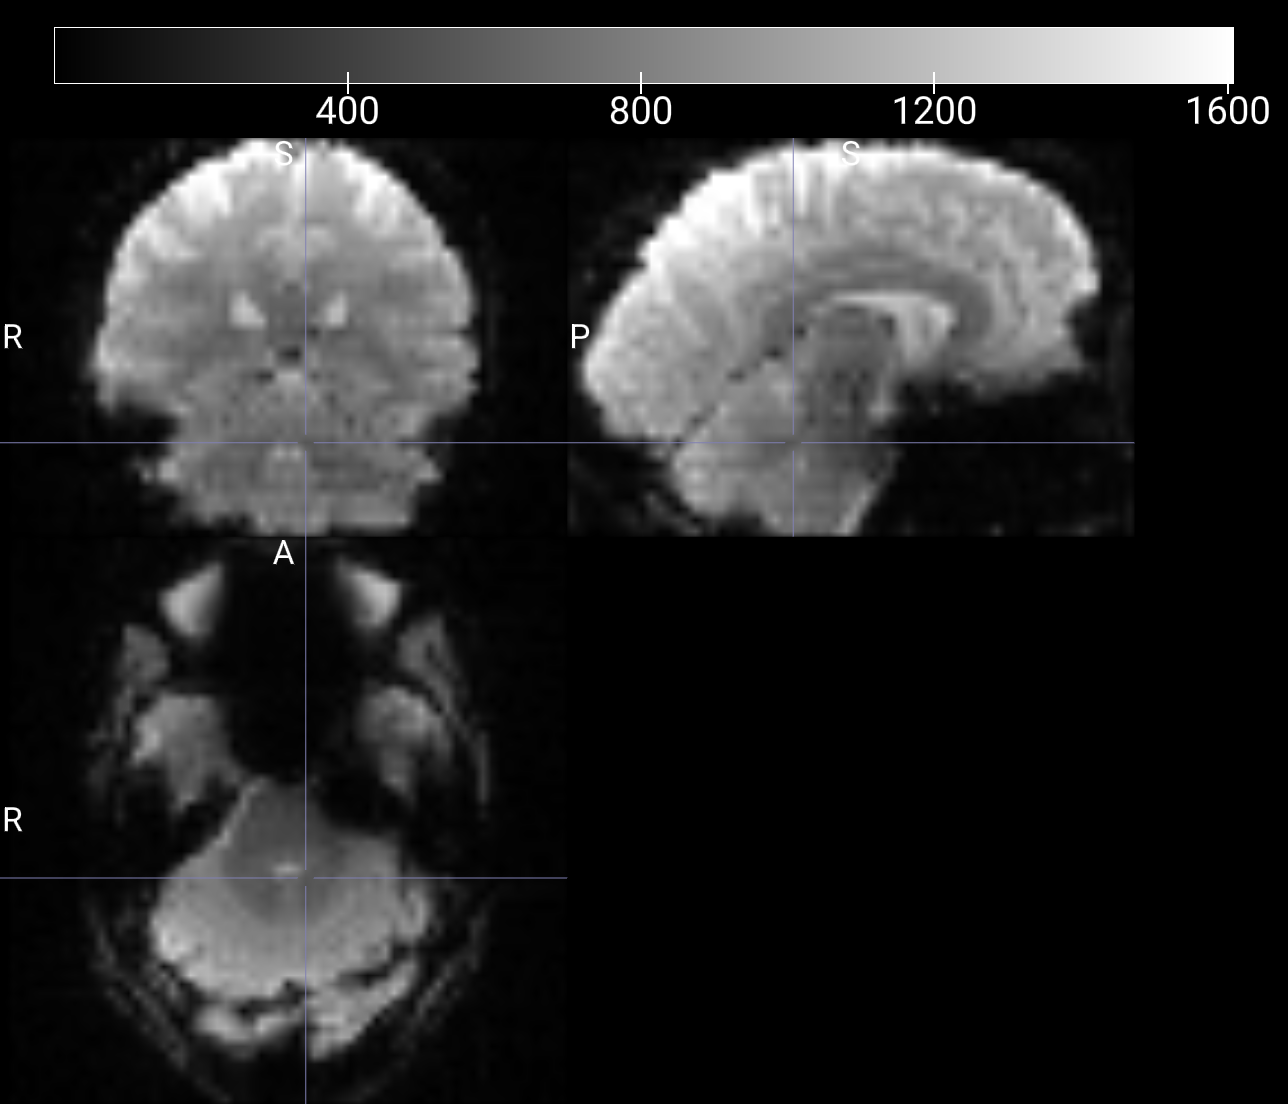
\includegraphics[width=\textwidth]{04_marco_teorico/images/bold_volume.png}
        \caption{Cortes de un volumen funcional (fMRI en estado de reposo).}
    \end{subfigure}

    \vspace{0.5em}

    \begin{subfigure}{0.85\textwidth}
        \centering
        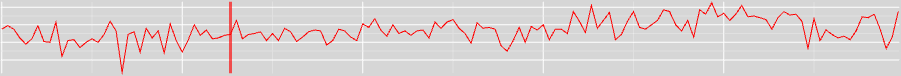
\includegraphics[width=\textwidth]{04_marco_teorico/images/bold_timeseries.png}
        \caption{Serie temporal de la señal BOLD correspondiente a un vóxel.}
    \end{subfigure}

    \caption{Ejemplo de señal BOLD en un vóxel. En la parte superior se muestran cortes del volumen funcional, y en la inferior la evolución temporal de la señal, que constituye la unidad básica para el análisis de conectividad funcional.}
    \label{fig:bold_parts}
\end{figure}


% 2.3
\section{Conectividad funcional en fMRI}
\label{sec:conectividad_funcional}

\subsection{Enfoque general de la conectividad funcional}

Como se describió en la Sección~\ref{sec:mri}, la resonancia magnética funcional permite observar la evolución temporal de la señal BOLD en distintas ubicaciones del cerebro. Cada vóxel queda asociado a una serie temporal que refleja variaciones en la oxigenación sanguínea a lo largo del tiempo.

Trabajar directamente a nivel vóxel implica manejar volúmenes tridimensionales con una cantidad muy grande de variables, lo cual resulta costoso desde el punto de vista computacional. Para dar una idea del orden de magnitud, una imagen cerebral típica tiene una resolución de aproximadamente $100 \times 100 \times 100$ vóxeles, es decir, del orden de $10^6$ variables. Si se quisiera calcular la correlación entre todos los pares de vóxeles, el número de conexiones crecería como el cuadrado del número de vóxeles, resultando en aproximadamente $10^{12}$ pares, lo cual es inviable en la práctica. Además, vóxeles espacialmente cercanos suelen presentar señales temporales similares, ya que capturan actividad proveniente de regiones anatómicamente próximas. Por este motivo, en muchos estudios no se pierde información relevante al resumir la señal a nivel regional, por ejemplo mediante el promedio de las señales de un conjunto de vóxeles que pertenecen a una misma zona.

En este contexto, la conectividad funcional se entiende como una forma de cuantificar la dependencia temporal entre regiones cerebrales anatómicamente separadas. Si las fluctuaciones de la señal BOLD de dos regiones tienden a variar de manera similar, o de forma opuesta, a lo largo del tiempo, se considera que existe conectividad funcional entre ellas \cite{van2010exploring}.

\subsection{Normalización espacial y parcelación cerebral}

Para poder comparar datos entre distintos sujetos, es necesario que las regiones cerebrales se correspondan de manera consistente entre individuos. Dado que cada cerebro presenta diferencias en forma y tamaño, en neuroimagen se utiliza un espacio de referencia común o espacio estándar que permita establecer una correspondencia anatómica entre sujetos.

Una estrategia ampliamente utilizada consiste en construir plantillas cerebrales a partir de imágenes de resonancia magnética de múltiples sujetos, las cuales son alineadas y promediadas para generar un cerebro de referencia. Un ejemplo clásico es la plantilla MNI152, construida a partir del promedio de imágenes T1 de 152 sujetos sanos por el Instituto Neurológico de Montreal. En esta plantilla, cada región anatómica se encuentra identificada con un nombre estándar, lo que permite que al transformar la imagen de un sujeto individual a este espacio de referencia, las distintas estructuras cerebrales queden asociadas de manera consistente a regiones conocidas y nombradas. Estas plantillas definen un espacio común que sirve como marco para el análisis de datos estructurales y funcionales.

En un pipeline típico de análisis, la imagen funcional se alinea espacialmente con la imagen estructural ponderada en T1 del mismo sujeto mediante un proceso de co-registración. Este paso permite que una misma región anatómica pueda identificarse de manera consistente tanto en la imagen estructural como en la funcional. Posteriormente, se aplican transformaciones espaciales (como traslaciones, rotaciones y deformaciones no lineales) para llevar ambos volúmenes al espacio estándar \cite{mandal2012structural}.

Una vez que los datos se encuentran en un espacio común, puede aplicarse un atlas o parcelación, que divide el cerebro en un conjunto finito de regiones etiquetadas. En este trabajo se utiliza el atlas \textit{Automated Anatomical Labeling} (AAL), ampliamente adoptado en estudios de neuroimagen \cite{tzourio2002automated}. El atlas AAL se encuentra disponible en distintas configuraciones; en la práctica, suele emplearse con 90 o 116 regiones. En este trabajo se utiliza la versión de 116 regiones, acorde a los datos analizados.

La Figura~\ref{fig:t1} muestra un ejemplo de imagen estructural ponderada en T1, que actúa como referencia anatómica para la co-registración de la imagen funcional y su posterior transformación al espacio estándar.

\begin{figure}[H]
    \centering
    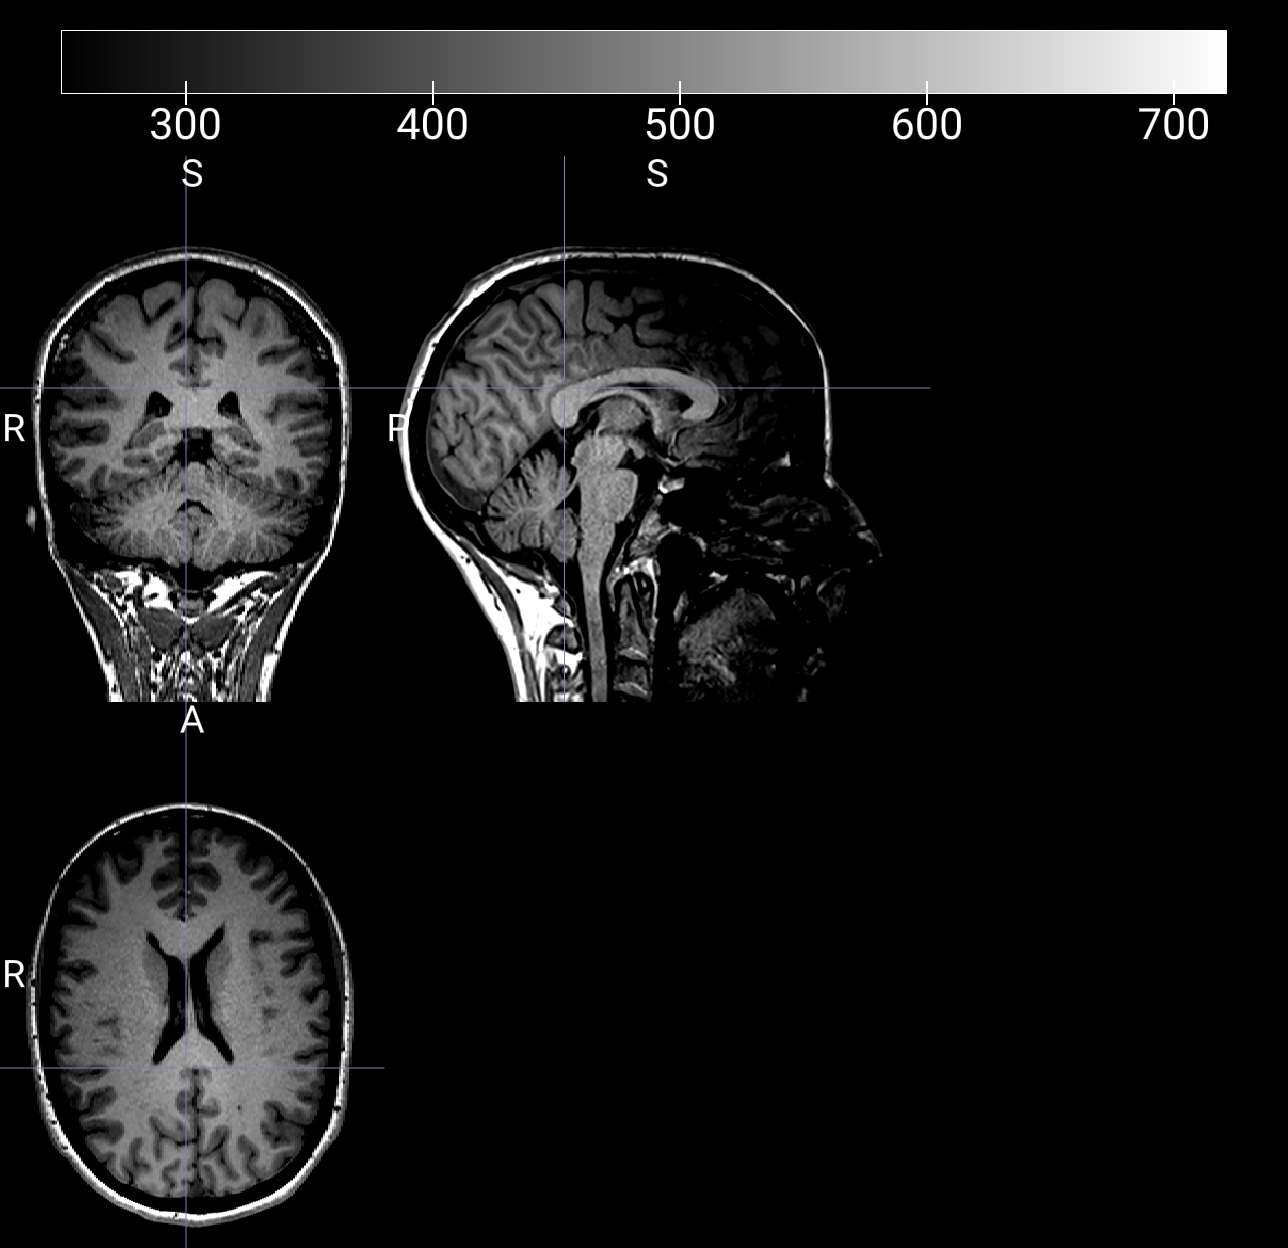
\includegraphics[width=0.85\textwidth]{04_marco_teorico/images/t1_structural.png}
    \caption{Ejemplo de imagen estructural ponderada en T1 (T1w) de un sujeto. Este volumen se utiliza como referencia anatómica para la co-registración de la imagen funcional y su posterior normalización al espacio estándar.}
    \label{fig:t1}
\end{figure}

La Figura~\ref{fig:mni} muestra el cerebro estándar MNI152 utilizado como referencia anatómica común para la alineación espacial entre sujetos. Sobre este espacio normalizado se aplica posteriormente la parcelación anatómica mediante el atlas AAL, como se ilustra en la Figura~\ref{fig:aal_mni}, donde cada color representa una región de interés (ROI) distinta.

\begin{figure}[H]
    \centering
    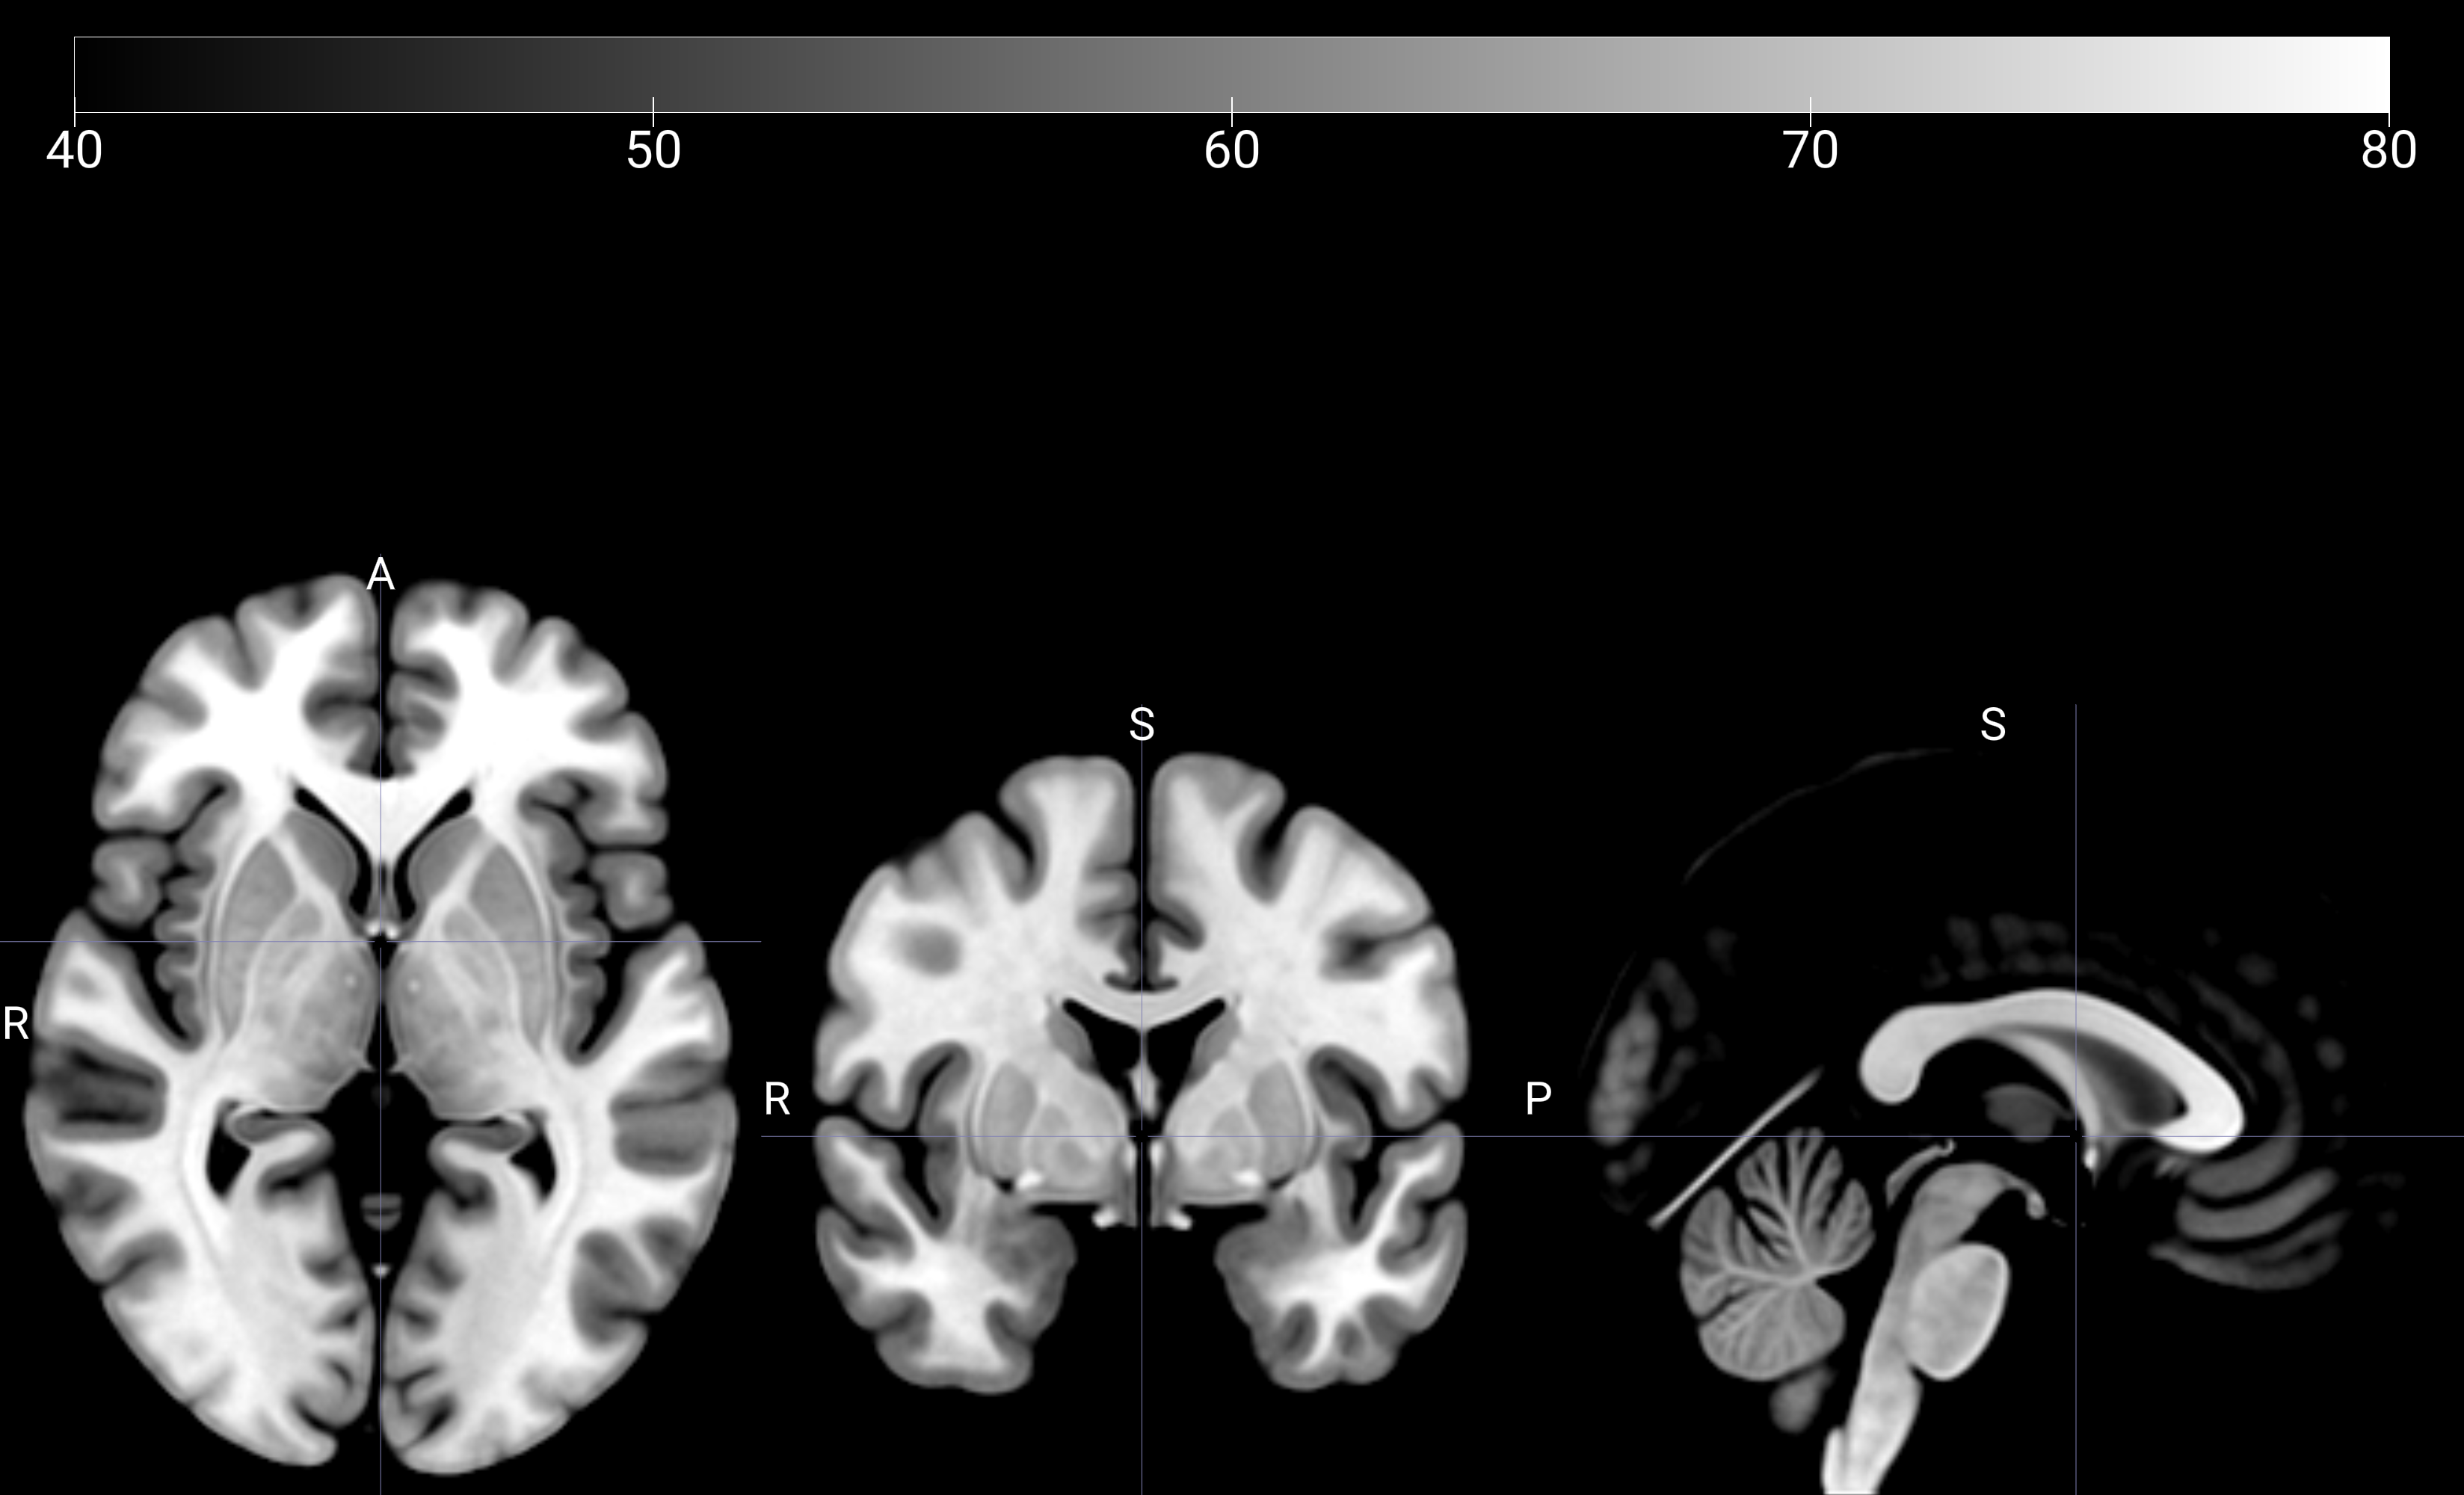
\includegraphics[width=0.85\textwidth]{04_marco_teorico/images/mni152.png}
    \caption{Cerebro estándar MNI152 en espacio normalizado, utilizado como referencia anatómica común para la alineación espacial entre sujetos.}
    \label{fig:mni}
\end{figure}

\begin{figure}[H]
    \centering
    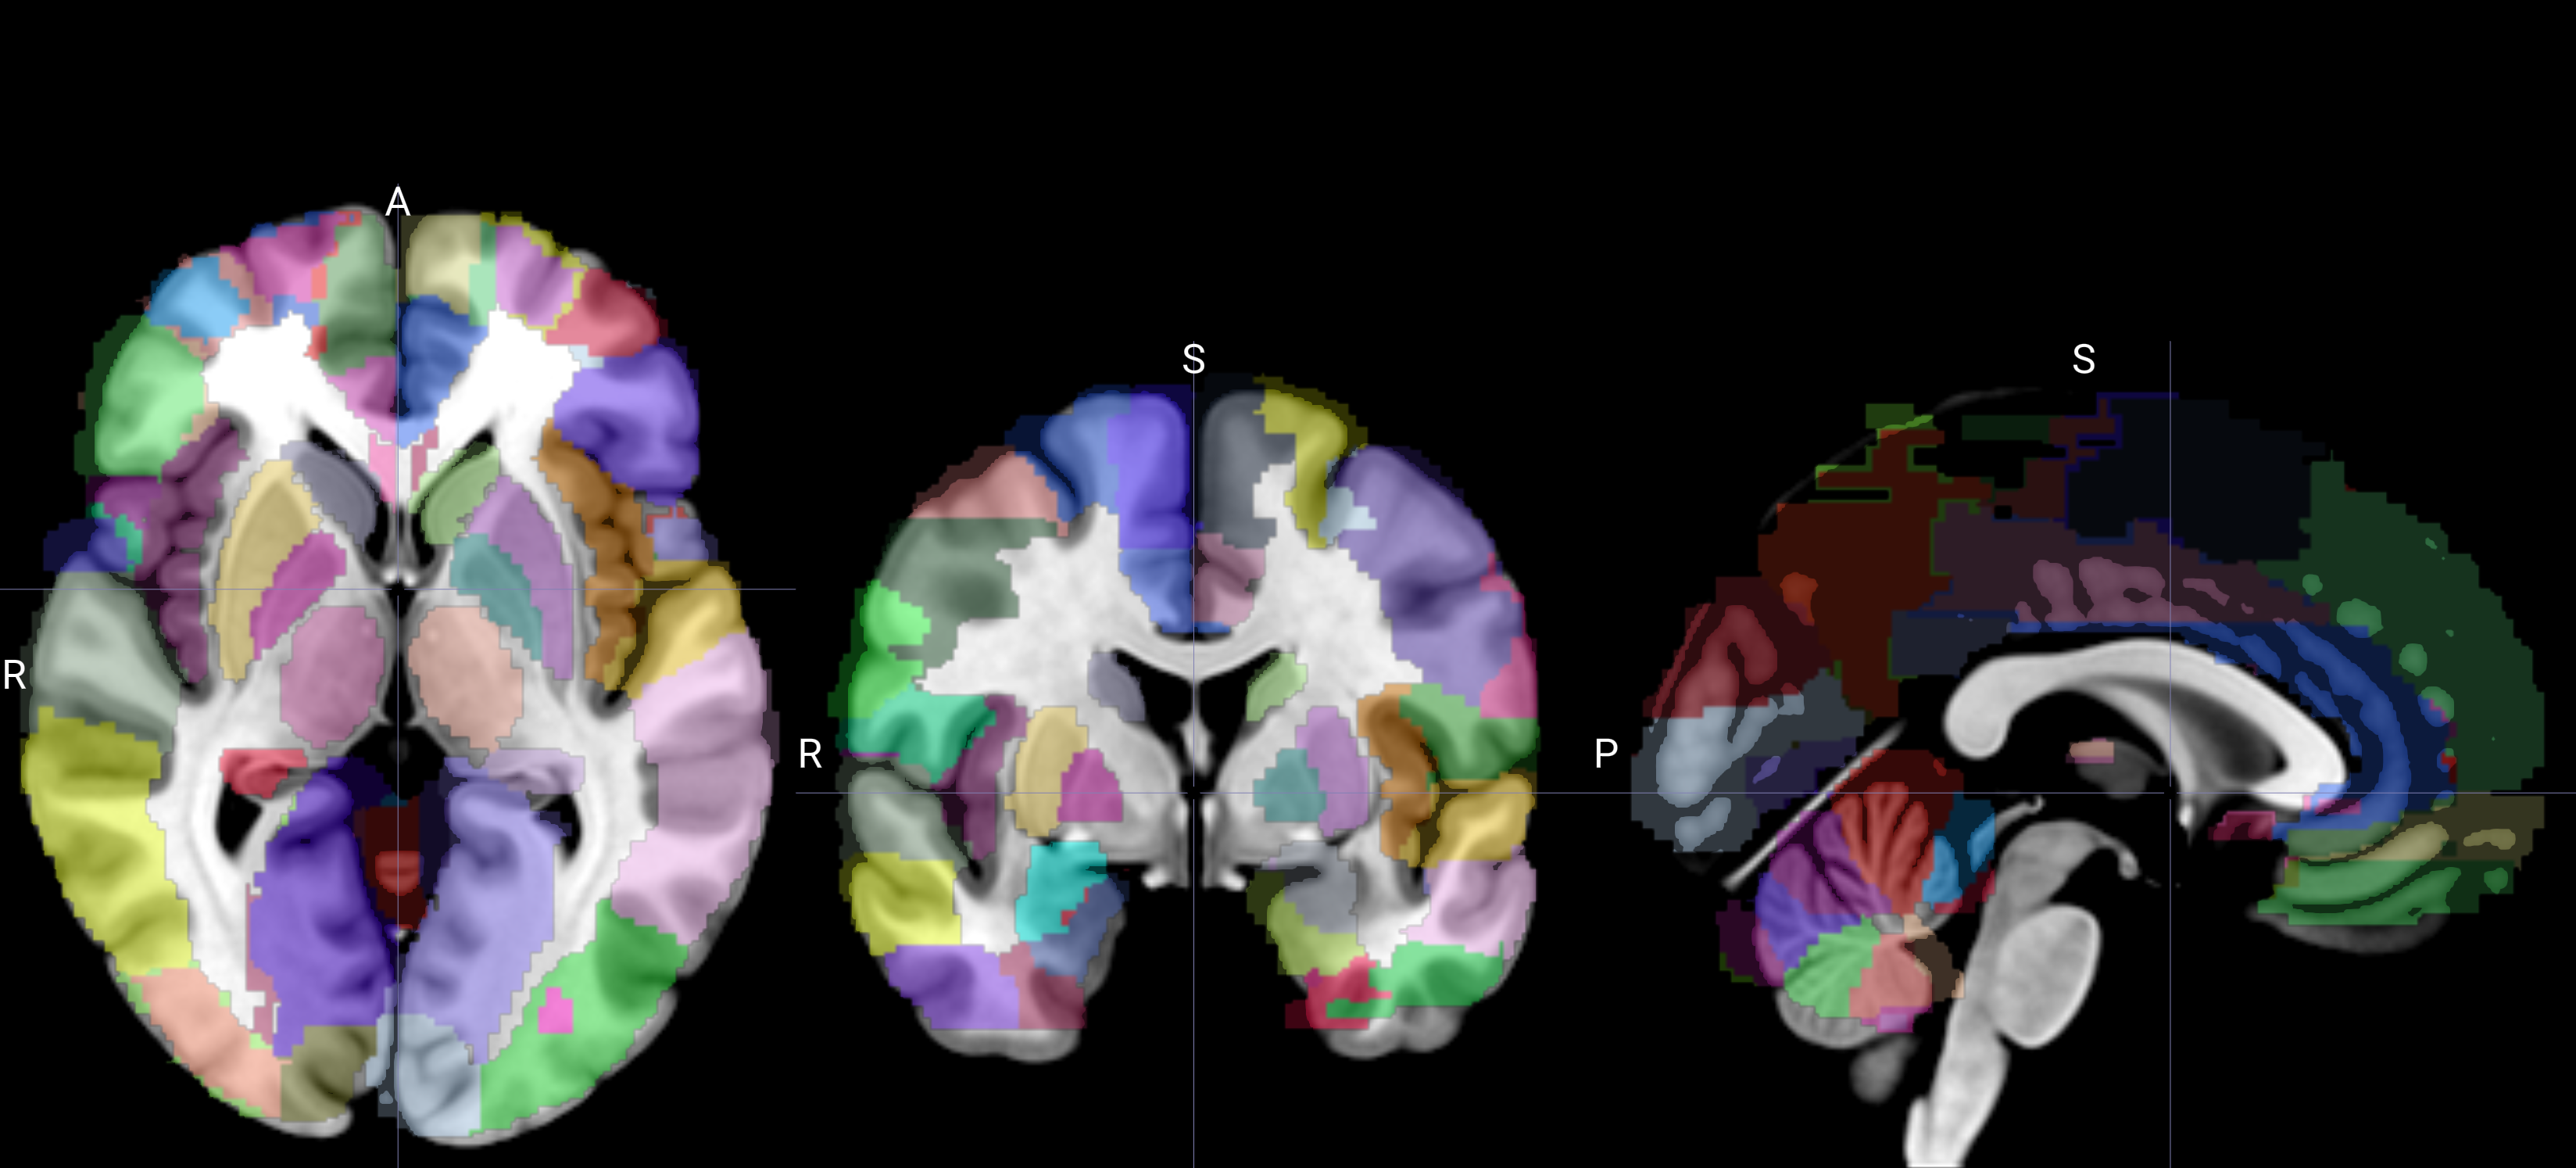
\includegraphics[width=0.85\textwidth]{04_marco_teorico/images/mni152+atlas.png}
    \caption{Atlas Automated Anatomical Labeling (AAL) superpuesto sobre el cerebro estándar MNI152. Cada color representa una región anatómica distinta utilizada como región de interés (ROI).}
    \label{fig:aal_mni}
\end{figure}


\subsection{Obtención de series temporales regionales}

Una vez aplicado el atlas, cada región agrupa múltiples vóxeles. Una forma habitual de representar la actividad de cada región consiste en construir una serie temporal regional como el promedio de las señales BOLD de los vóxeles pertenecientes a dicha región. Este procedimiento reduce significativamente la dimensionalidad de los datos y facilita el análisis posterior, manteniendo información relevante sobre la dinámica temporal de la señal \cite{shahhosseini2022functional}.

En estudios de fMRI en estado de reposo, la señal BOLD suele someterse a distintos pasos de preprocesamiento con el objetivo de reducir fuentes de ruido y mejorar la comparabilidad entre sujetos. Estos pasos incluyen correcciones asociadas al movimiento del sujeto durante la toma de imágenes, regresión de señales no neuronales y filtrado temporal. En particular, se ha observado que las fluctuaciones relevantes de la señal en estado de reposo se concentran en un rango de bajas frecuencias, típicamente del orden de 0,01–0,08 Hz \cite{smitha2017resting}.

En este trabajo se parte directamente de series temporales regionales que ya fueron obtenidas y preprocesadas como parte del procesamiento previo de los datos, por lo que no se realizan pasos adicionales de preprocesamiento a nivel vóxel.

\subsection{Estimación y representación de la conectividad funcional}

Con una serie temporal por región, la conectividad funcional se estima midiendo la dependencia estadística entre pares de regiones. Una de las medidas más utilizadas para este fin es la correlación de Pearson, debido a su simplicidad e interpretabilidad, ya que cuantifica el grado de asociación lineal entre dos series temporales \cite{van2010exploring}. Esta medida permite evaluar si dos regiones presentan fluctuaciones temporales sincronizadas o anticorrelacionadas.

La Figura~\ref{fig:ts_corr} ilustra este concepto con dos ejemplos: un par de regiones cuyas señales fluctúan de forma sincronizada (correlación positiva alta) y un par con fluctuaciones opuestas (anticorrelación).

\begin{figure}[H]
    \centering
    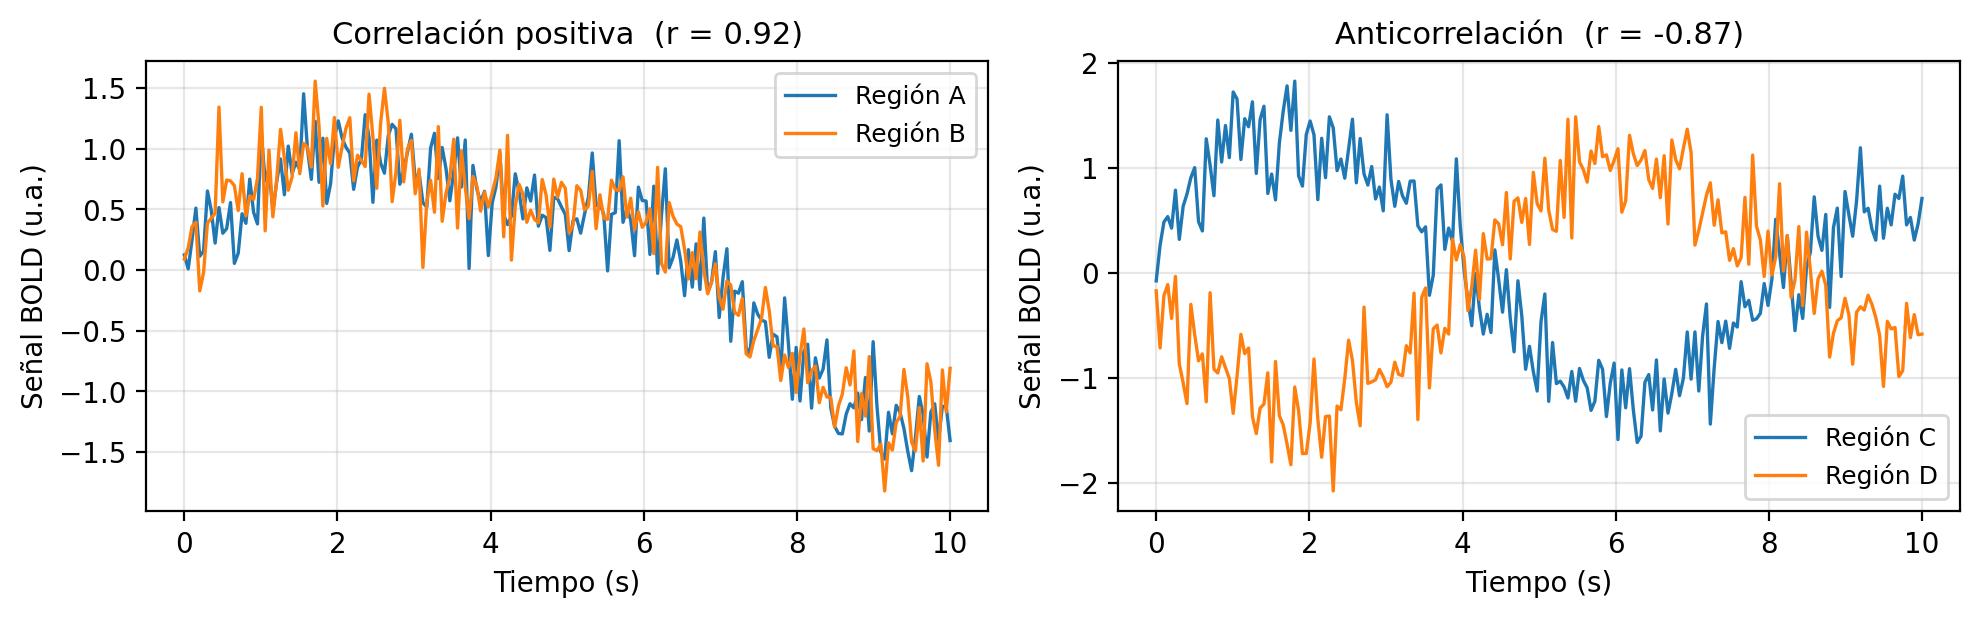
\includegraphics[width=0.95\textwidth]{04_marco_teorico/images/timeseries_correlation.png}
    \caption{Ejemplo de series temporales BOLD simuladas para dos pares de regiones cerebrales. Izquierda: regiones con correlación positiva ($r = 0{,}92$), cuyas señales fluctúan de forma sincronizada. Derecha: regiones anticorrelacionadas ($r = -0{,}87$), con fluctuaciones opuestas.}
    \label{fig:ts_corr}
\end{figure}

A partir de estas correlaciones se construye una matriz de conectividad funcional de tamaño $N \times N$, donde $N$ es el número de regiones del atlas. Cada entrada $(i,j)$ corresponde a la correlación entre la serie temporal regional de la región $i$ y la de la región $j$. Esta representación matricial constituye una forma compacta y ampliamente utilizada de describir la organización funcional del cerebro, y sirve como punto de partida para análisis posteriores basados en redes o enfoques de aprendizaje automático.

La Figura~\ref{fig:fc} muestra un ejemplo de una matriz de conectividad funcional real obtenida a partir de datos de fMRI en estado de reposo, ilustrando la estructura simétrica y los patrones de asociación entre regiones.

\begin{figure}[H]
    \centering
    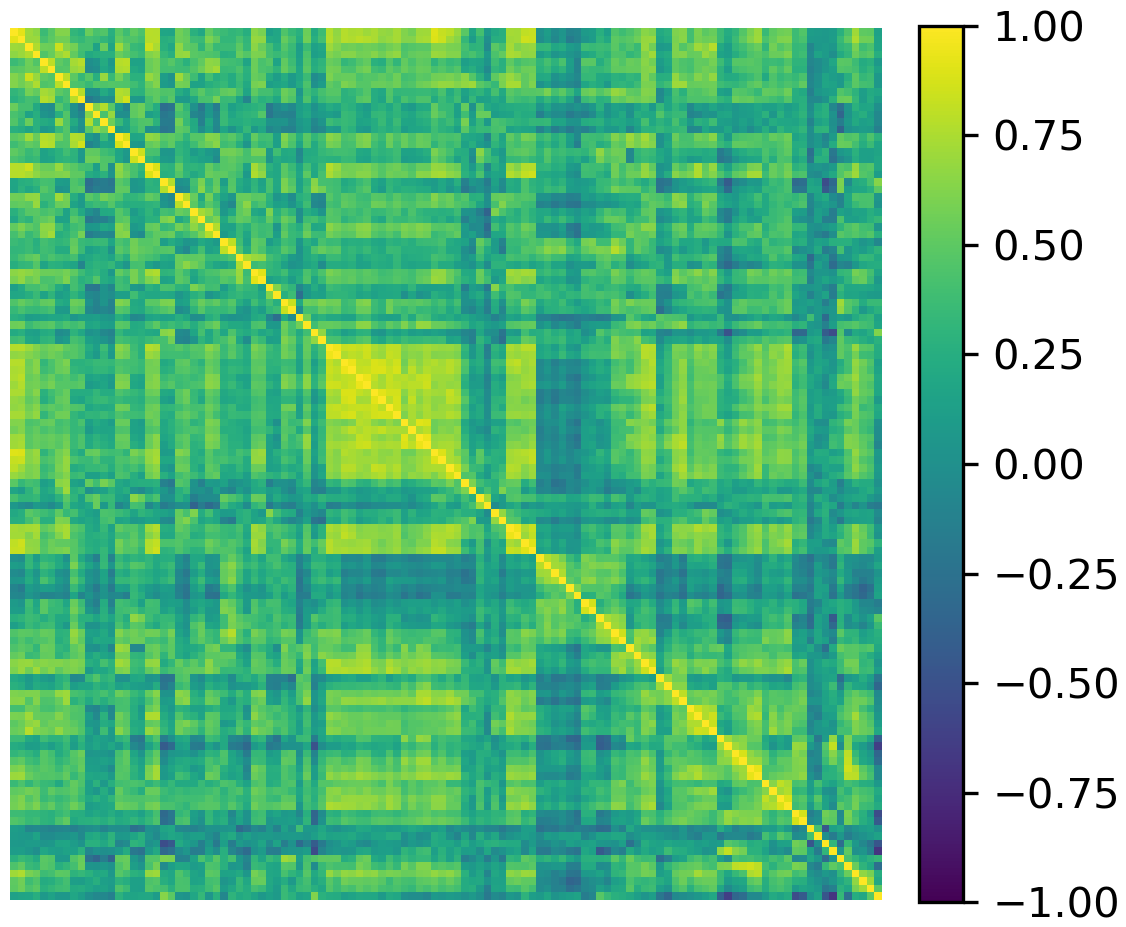
\includegraphics[width=0.6\textwidth]{04_marco_teorico/images/fc_example.png}
    \caption{Ejemplo de matriz de conectividad funcional (116×116) estimada mediante correlación de Pearson entre las series temporales regionales. Cada entrada representa el grado de asociación entre dos regiones cerebrales.}
    \label{fig:fc}
\end{figure}

\subsection{Transformación Fisher $z$}
\label{sec:fisher_z}

Los coeficientes de correlación de Pearson están acotados al intervalo $(-1, 1)$ y presentan una distribución asimétrica, particularmente para valores cercanos a los extremos. Esta propiedad puede resultar problemática para métodos estadísticos y modelos de aprendizaje automático que asumen distribuciones aproximadamente normales.

La transformación Fisher $z$ \cite{fisher1921probable} convierte los coeficientes de correlación en valores definidos sobre toda la recta real con una distribución aproximadamente normal:
\[
z_{ij} = \text{arctanh}(r_{ij}) = \frac{1}{2} \ln \left( \frac{1 + r_{ij}}{1 - r_{ij}} \right),
\]
donde $r_{ij}$ es la correlación de Pearson entre las regiones $i$ y $j$. Esta transformación es una práctica estándar en estudios de conectividad funcional y tiene la ventaja adicional de estabilizar la varianza de los coeficientes de correlación, lo que favorece la estabilidad numérica durante el entrenamiento de modelos.

%2.4

\section{Modelos computacionales y aprendizaje automático}
\label{sec:modelos_ml}

\subsection{Aprendizaje automático en neuroimagen}
Durante las últimas décadas se han producido avances significativos en el estudio del cerebro y de los trastornos neurológicos y psiquiátricos, en gran parte impulsados por el desarrollo de técnicas de neuroimagen. Tradicionalmente, el análisis de estos datos se ha basado en métodos estadísticos clásicos orientados a realizar inferencias a nivel grupal. Este enfoque consiste, en general, en comparar grupos de sujetos (por ejemplo, pacientes y controles sanos) para identificar diferencias promedio en determinadas regiones o medidas cerebrales.

Si bien estos métodos han permitido caracterizar patrones generales asociados a distintas patologías, presentan limitaciones importantes cuando se pretende realizar inferencias a nivel individual. En particular, los análisis grupales no permiten realizar predicciones sobre sujetos individuales, lo que ha dificultado la transferencia de los resultados de la investigación en neuroimagen hacia aplicaciones clínicas, como el diagnóstico personalizado o la predicción de respuesta a tratamientos \cite{mwangi2014review}.

En este contexto, el aprendizaje automático ha emergido como una herramienta clave para el análisis de datos de neuroimagen. A diferencia de los enfoques clásicos, los métodos de aprendizaje automático permiten identificar patrones complejos en los datos que distinguen sujetos sanos de pacientes, o bien subgrupos de pacientes con características clínicas diferentes. Estos métodos han demostrado ser capaces de realizar predicciones a nivel individual (es decir, estimar una variable de interés para cada sujeto por separado, en contraste con la comparación de promedios entre grupos), abriendo nuevas posibilidades para el desarrollo de herramientas de apoyo al diagnóstico y a la toma de decisiones clínicas \cite{vieira2020introduction}. Cabe señalar que esto no impide que los modelos se entrenen sobre cohortes heterogéneas que incluyan tanto sujetos sanos como pacientes; la diferencia radica en que la predicción se realiza para cada individuo.

Otra diferencia fundamental radica en el carácter multivariable del aprendizaje automático. Mientras que los enfoques estadísticos tradicionales suelen analizar una variable a la vez, los modelos de aprendizaje automático consideran simultáneamente un gran número de variables de entrada. Esto resulta especialmente relevante en neuroimagen, donde es frecuente combinar información proveniente de múltiples modalidades, como imágenes estructurales, funcionales o de difusión, con el objetivo de mejorar el poder predictivo de los modelos \cite{mwangi2014review}.

Desde un punto de vista conceptual, el objetivo del análisis también se desplaza. En lugar de formular hipótesis específicas sobre los datos y evaluarlas bajo supuestos estadísticos predefinidos, el aprendizaje automático adopta un enfoque más exploratorio, en el cual se busca que los propios datos revelen patrones y relaciones relevantes sin imponer restricciones fuertes a priori \cite{vieira2020introduction}.

\subsection{Motivación para la reducción de dimensionalidad}
Un desafío central en la aplicación de aprendizaje automático a datos de neuroimagen es la alta dimensionalidad de los datos. En muchos estudios, el número de sujetos disponibles suele ser relativamente pequeño, mientras que el número de variables (por ejemplo, vóxeles o características derivadas de las imágenes) puede superar ampliamente las decenas o cientos de miles. Esta situación, conocida como el problema de alta dimensionalidad o ``small-n large-p'', incrementa significativamente el riesgo de sobreajuste de los modelos \cite{mwangi2014review}.

El sobreajuste ocurre cuando un modelo aprende patrones específicos del conjunto de entrenamiento que no generalizan a nuevos datos, lo que se traduce en un bajo rendimiento predictivo sobre sujetos no vistos durante el entrenamiento. Para mitigar este problema, existe un amplio consenso en la literatura de neuroimagen sobre la necesidad de aplicar técnicas de reducción de dimensionalidad o selección de características antes de entrenar modelos predictivos \cite{mwangi2014review}.

Además de reducir el riesgo de sobreajuste y el costo computacional, la reducción de dimensionalidad puede contribuir a eliminar información redundante o irrelevante y facilitar una interpretación más clara de los patrones subyacentes en los datos. En este sentido, los métodos de reducción de dimensionalidad constituyen un componente fundamental en muchos pipelines de aprendizaje automático aplicados a neuroimagen.

Entre los métodos de reducción de dimensionalidad más utilizados se encuentran el Análisis de Componentes Principales (PCA), un enfoque lineal clásico, y los autoencoders variacionales, capaces de modelar relaciones no lineales. Ambos enfoques se describen a continuación.


\subsection{Análisis de Componentes Principales (PCA)}
\label{sec:pca}

El Análisis de Componentes Principales (\textit{Principal Component Analysis}, PCA) es uno de los métodos de reducción de dimensionalidad más utilizados en estadística y aprendizaje automático \cite{jolliffe2002pca}. Su objetivo es transformar un conjunto de variables posiblemente correlacionadas en un nuevo conjunto de variables no correlacionadas, denominadas \textit{componentes principales}, que resumen la información más relevante contenida en los datos originales.

La intuición detrás de PCA es sencilla: dado un conjunto de datos de alta dimensionalidad, muchas de las variables originales están correlacionadas entre sí y contienen información redundante. PCA identifica las direcciones en el espacio de datos a lo largo de las cuales la variabilidad es máxima, es decir, las direcciones que mejor distinguen entre las observaciones. La primera componente principal es la dirección de mayor varianza; la segunda es la dirección de mayor varianza restante, con la restricción de ser perpendicular a la primera; y así sucesivamente. De esta forma, las primeras $k$ componentes capturan la mayor parte de la variabilidad total de los datos, y las restantes (que contienen principalmente ruido o información redundante) pueden descartarse.

Desde el punto de vista práctico, aplicar PCA equivale a proyectar los datos originales sobre estas $k$ direcciones principales, obteniendo una representación compacta donde cada observación queda descrita por $k$ valores en lugar de los $p$ originales. Por ejemplo, en el contexto de este trabajo, una matriz de conectividad funcional representada por 6670 valores puede comprimirse a 64 componentes principales, reteniendo las fuentes de variación más informativas y descartando el resto.

PCA es un método determinista y lineal: solo puede capturar relaciones lineales entre las variables originales. Esta limitación, que lo distingue de los autoencoders (capaces de modelar dependencias no lineales), tiene como contrapartida una notable simplicidad: PCA no requiere entrenamiento iterativo, no tiene hiperparámetros más allá del número de componentes $k$, y su cálculo se obtiene directamente a partir de la estructura de covarianza de los datos \cite{jolliffe2002pca}. En el contexto de neuroimagen, PCA y sus extensiones han sido utilizados como componente de reducción de dimensionalidad en pipelines de predicción de edad cerebral a partir de conectividad funcional \cite{monti2020interpretable}, y comparaciones sistemáticas de workflows han identificado a PCA combinado con algoritmos no lineales entre las configuraciones de mejor rendimiento \cite{more2023brain}.

\subsection{Autoencoders y autoencoders variacionales}

\subsubsection{Autoencoders}

Un autoencoder es un tipo de red neuronal multicapa entrenada con el objetivo de reproducir su entrada en la salida. Su arquitectura se compone de dos módulos principales: un codificador (\textit{encoder}), que transforma los datos de entrada en una representación de menor dimensión, y un decodificador (\textit{decoder}), que intenta reconstruir la entrada original a partir de dicha representación \cite{vieira2017using,michelucci2022introduction}.

El codificador aprende una representación latente para cada dato de entrada, expresada como un vector en un espacio latente de dimensión reducida. Esta representación puede interpretarse como un punto en un espacio multidimensional de menor dimensión que el espacio original. De este modo, una entrada originalmente descrita por un gran número de variables es transformada en una representación compacta que captura patrones o información relevante de los datos originales.

Desde el punto de vista del aprendizaje, los autoencoders se entrenan de manera no supervisada, ya que no requieren datos etiquetados. El propio conjunto de datos de entrada actúa como referencia durante el entrenamiento, dado que el objetivo del modelo es minimizar la diferencia entre la entrada y su reconstrucción. Esta diferencia se cuantifica mediante un error de reconstrucción, que mide qué tan fiel es la salida del modelo con respecto al dato original. Una de las métricas más utilizadas para este fin es el error cuadrático medio (MSE), definido como
\[
MSE = \frac{1}{N} \sum_{i=1}^{N} (x_i - \tilde{x}_i)^2.
\]
Un valor elevado del error de reconstrucción indica que el modelo no ha logrado capturar adecuadamente la estructura de los datos, mientras que un valor reducido sugiere que la representación latente aprendida permite reconstrucciones precisas \cite{michelucci2022introduction}. Otra métrica frecuente es el error absoluto medio (MAE), más robusta ante valores atípicos. En este trabajo se utiliza MAE como pérdida de reconstrucción (véase Capítulo~\ref{chapter:metodologia_pipeline}).

Una característica fundamental de los autoencoders es la presencia de un cuello de botella (\textit{bottleneck}) en el espacio latente, que fuerza al modelo a reducir progresivamente la dimensionalidad de los datos a través de capas intermedias con un número decreciente de unidades. Esta restricción obliga al modelo a aprender representaciones informativas, ya que solo puede preservar la información más relevante para reconstruir adecuadamente la entrada. Por este motivo, los autoencoders son utilizados frecuentemente como extractores de características en distintos contextos, incluyendo aplicaciones de neuroimagen \cite{vieira2017using}.

La dimensionalidad del espacio latente constituye un compromiso central en el diseño de un autoencoder. Un espacio latente excesivamente pequeño puede limitar la capacidad del modelo para capturar características relevantes de los datos, lo que se traduce en reconstrucciones imprecisas. Por el contrario, un espacio latente demasiado grande puede reducir la efectividad del cuello de botella, permitiendo representaciones poco informativas y afectando la organización del espacio latente. En la práctica, una mala calidad de reconstrucción suele estar asociada a un espacio latente desestructurado, donde las representaciones aprendidas no reflejan adecuadamente las relaciones entre los datos.

En comparación con PCA (Sección~\ref{sec:pca}), los autoencoders presentan ciertas ventajas prácticas. En particular, pueden entrenarse utilizando mini-batches, lo que los hace adecuados para trabajar con grandes volúmenes de datos, mientras que PCA requiere procesar el conjunto completo de datos para estimar la transformación. Además, al utilizar funciones de activación no lineales, los autoencoders pueden modelar relaciones más complejas entre las variables de entrada, lo que puede resultar beneficioso en contextos donde los datos presentan estructuras no triviales. Sin embargo, esta mayor expresividad tiene un costo: los autoencoders introducen múltiples hiperparámetros (número de capas, dimensiones, tasa de aprendizaje, regularización) que requieren ser optimizados, mientras que PCA solo requiere la elección del número de componentes $k$.

La Figura~\ref{fig:ae_arch} esquematiza la arquitectura general de un autoencoder convencional.

\begin{figure}[H]
\centering
\shorthandoff{>}
\begin{tikzpicture}[
    >=Stealth,
    neuron/.style={circle, draw, thick, minimum size=0.55cm, inner sep=0pt},
    input/.style={neuron, fill=teal!20},
    hidden/.style={neuron, fill=blue!15},
    latent/.style={neuron, fill=orange!25},
    output/.style={neuron, fill=teal!20},
    conn/.style={-, gray!50, thin},
    arr/.style={->, thick},
    brace/.style={decorate, decoration={brace, amplitude=5pt, mirror}},
]

% --- Input layer (5 neurons) ---
\foreach \i in {1,...,5} {
    \node[input] (in\i) at (0, -\i*0.8 + 2.4) {};
}
\node[above=0.15cm of in1, font=\small\bfseries] {$\mathbf{x}$};

% --- Encoder hidden layer (3 neurons) ---
\foreach \i in {1,...,3} {
    \node[hidden] (h1\i) at (2.2, -\i*0.8 + 1.6) {};
}

% --- Latent layer (2 neurons) ---
\foreach \i in {1,...,2} {
    \node[latent] (z\i) at (4.4, -\i*0.8 + 1.2) {};
}
\node[above=0.15cm of z1, font=\small\bfseries] {$\mathbf{z}$};
\node[below=0.3cm of z2, font=\footnotesize, gray] (kdims) {$k$ dims};

% --- Decoder hidden layer (3 neurons) ---
\foreach \i in {1,...,3} {
    \node[hidden] (h2\i) at (6.6, -\i*0.8 + 1.6) {};
}

% --- Output layer (5 neurons) ---
\foreach \i in {1,...,5} {
    \node[output] (out\i) at (8.8, -\i*0.8 + 2.4) {};
}
\node[above=0.15cm of out1, font=\small\bfseries] {$\tilde{\mathbf{x}}$};

% --- Connections: input -> hidden1 ---
\foreach \i in {1,...,5} {
    \foreach \j in {1,...,3} {
        \draw[conn] (in\i) -- (h1\j);
    }
}
% --- Connections: hidden1 -> latent ---
\foreach \i in {1,...,3} {
    \foreach \j in {1,...,2} {
        \draw[conn] (h1\i) -- (z\j);
    }
}
% --- Connections: latent -> hidden2 ---
\foreach \i in {1,...,2} {
    \foreach \j in {1,...,3} {
        \draw[conn] (z\i) -- (h2\j);
    }
}
% --- Connections: hidden2 -> output ---
\foreach \i in {1,...,3} {
    \foreach \j in {1,...,5} {
        \draw[conn] (h2\i) -- (out\j);
    }
}

% --- Braces and labels ---
\draw[decorate, decoration={brace, amplitude=5pt}]
    (-0.65, -2.0) -- (-0.65, 2.0)
    node[midway, left=6pt, font=\footnotesize, align=center] {$d$\\dims};
\draw[decorate, decoration={brace, amplitude=5pt, mirror}]
    (9.45, -2.0) -- (9.45, 2.0)
    node[midway, right=6pt, font=\footnotesize, align=center] {$d$\\dims};

% --- Encoder / Decoder labels ---
\node[font=\footnotesize, gray] at (1.1, -2.8) {Encoder};
\node[font=\footnotesize, gray] at (7.7, -2.8) {Decoder};
\draw[gray, dashed, rounded corners] (-0.6, -2.5) rectangle (5.0, 2.8);
\draw[gray, dashed, rounded corners] (3.8, -2.5) rectangle (9.4, 2.8);

% --- Latent space mini-plot ---
\begin{scope}[shift={(4.4, -4.2)}]
    % Axes
    \draw[->, thick] (-1.1, 0) -- (1.3, 0) node[right, font=\scriptsize] {$z_1$};
    \draw[->, thick] (0, -0.9) -- (0, 1.3) node[above, font=\scriptsize] {$z_2$};
    % Scattered points (other data points, light)
    \foreach \px/\py in {-0.7/0.3, -0.4/-0.5, 0.2/0.8, 0.6/-0.3, 0.9/0.5,
                         -0.3/0.7, 0.5/0.1, -0.8/-0.2, 0.1/-0.7, 0.7/0.9} {
        \fill[blue!25] (\px, \py) circle (1.5pt);
    }
    % Highlighted point
    \fill[orange!80!red] (0.35, 0.45) circle (3pt);
    \draw[-{Stealth[length=1.8mm]}, orange!80!red, semithick] (0.47, 0.53) -- ++(0.25, 0.18)
        node[right, font=\scriptsize] {$\mathbf{z}_i$};
    % Label
    \node[below=0.2cm, font=\scriptsize, gray] at (0, -0.9) {Espacio latente};
\end{scope}

% --- Arrow from latent neurons to mini-plot ---
\draw[->, dashed, gray] (kdims.south) -- ++(0, -0.8);

% --- Loss below ---
\node[font=\small] at (4.4, -6.5) {$\mathcal{L}_{\text{rec}}(\mathbf{x}, \tilde{\mathbf{x}})$};

\end{tikzpicture}
\shorthandon{>}
\caption{Arquitectura de un autoencoder convencional. La entrada $\mathbf{x}$ de dimensión $d$ es comprimida por el encoder a trav\'es de capas ocultas sucesivamente menores hasta una representación latente $\mathbf{z}$ de baja dimensión (cuello de botella). El decoder reconstruye la entrada original como $\tilde{\mathbf{x}}$. El mini-gráfico inferior ilustra el espacio latente bidimensional, donde cada punto naranja representa la codificación de un dato de entrada. El modelo se entrena minimizando $\mathcal{L}_{\text{rec}}$.}
\label{fig:ae_arch}
\end{figure}

\subsubsection{Autoencoders variacionales (VAE)}

Los autoencoders clásicos, si bien efectivos para reducir dimensionalidad, no imponen restricciones explícitas sobre la organización global del espacio latente. Como consecuencia, dicho espacio puede resultar irregular o fragmentado, de modo que tomar puntos arbitrarios y decodificarlos conduce, en muchos casos, a reconstrucciones poco significativas o dominadas por ruido. Idealmente, sería deseable que puntos cercanos en el espacio latente correspondan a datos similares, y que interpolaciones suaves entre representaciones latentes produzcan variaciones plausibles de los datos originales \cite{doersch2016tutorial}.

Los autoencoders variacionales (VAE) fueron propuestos originalmente por Kingma y Welling en el trabajo \textit{Auto-Encoding Variational Bayes} \cite{kingma2013auto} con el objetivo de abordar esta limitación mediante la introducción de una formulación probabilística del espacio latente. A diferencia de los autoencoders clásicos, que codifican cada entrada en un único vector latente determinista, un VAE asocia a cada dato de entrada $x$ una distribución de probabilidad sobre variables latentes $z$. Esta representación probabilística introduce incertidumbre controlada y permite imponer una estructura explícita sobre el espacio latente, favoreciendo su regularidad y continuidad \cite{kingma2019introduction}.

En este marco, se define una distribución latente $p(z)$, denominada \textit{prior}, a partir de la cual se busca generar representaciones latentes que luego puedan decodificarse para obtener observaciones en el espacio de datos. En términos generales, el objetivo de un VAE es aprender un modelo generativo capaz de producir datos plausibles similares a los observados en el conjunto de entrenamiento. Sin embargo, la distribución real de los datos $p(x)$ es desconocida y solo se dispone de muestras observadas, lo que impide su modelado directo \cite{kingma2019introduction}.

Para conectar el espacio latente con el espacio de datos, se consideran dos distribuciones condicionales. Por un lado, la distribución de verosimilitud $p(x|z)$ modela la probabilidad de observar un dato $x$ dado un vector latente $z$, y puede interpretarse como el mecanismo de decodificación desde el espacio latente hacia el espacio original. Por otro lado, la distribución posterior $p(z|x)$ describe qué valores latentes son compatibles con un dato observado $x$. En la práctica, esta distribución posterior resulta intratable, por lo que se introduce un modelo de inferencia aproximado $q(z|x)$, también denominado codificador o modelo de reconocimiento, que aproxima la posterior verdadera \cite{kingma2019introduction,doersch2016tutorial}.

En los VAEs se asume habitualmente un prior simple y conocido, típicamente una distribución normal estándar,
\[
p(z) = \mathcal{N}(0, I),
\]
y se aproxima la posterior mediante una distribución gaussiana cuyos parámetros dependen de la entrada:
\[
q(z|x) = \mathcal{N}\big(\mu(x), \sigma^2(x)\big).
\]
De este modo, el codificador no produce directamente un único vector latente determinista, sino los parámetros $\mu(x)$ y $\sigma(x)$ que definen una distribución latente asociada a cada dato. Esta distribución constituye la representación latente del dato en el VAE. A partir de ella, se obtiene un vector latente $z$ mediante muestreo, que es utilizado por el decodificador para reconstruir o generar una salida $\tilde{x}$.


Desde el punto de vista de la optimización, el entrenamiento de un VAE no se limita a minimizar una pérdida de reconstrucción, como ocurre en los autoencoders clásicos. La función objetivo incorpora además un término de regularización que promueve que la distribución latente aproximada $q(z|x)$ permanezca cercana al prior $p(z)$. Este término se expresa mediante la divergencia de Kullback--Leibler (KL), que mide la discrepancia entre dos distribuciones de probabilidad. La combinación de ambos objetivos se formaliza a través del criterio conocido como \textit{Evidence Lower Bound} (ELBO), que permite entrenar el modelo equilibrando la calidad de la reconstrucción con la regularización del espacio latente \cite{kingma2013auto}.
\[
\mathcal{L}_{VAE} =
\mathcal{L}_{rec}(x, \tilde{x}) +
D_{KL}\big(q(z|x)\,\|\,p(z)\big).
\]
La pérdida de reconstrucción $\mathcal{L}_{rec}$ evalúa qué tan fiel es la reconstrucción respecto a la entrada original, mientras que el término KL actúa como regularizador del espacio latente, favoreciendo representaciones continuas y bien organizadas \cite{doersch2016tutorial}.

Un aspecto fundamental en el entrenamiento de los VAEs es que la obtención del vector latente implica un proceso de muestreo, lo cual introduce aleatoriedad en el flujo de cómputo. En particular, cuando el vector latente se obtiene muestreando directamente de una distribución cuyos parámetros dependen de la entrada, dicha operación deja de ser una función determinista de los parámetros del modelo. Esto impide la propagación directa de gradientes, ya que el muestreo no es una operación diferenciable respecto a dichos parámetros.

Para resolver este inconveniente, se utiliza el denominado truco de reparametrización, que permite separar la fuente de aleatoriedad de los parámetros del modelo y expresar el muestreo de manera diferenciable \cite{kingma2013auto}. En lugar de muestrear directamente desde la distribución latente, se introduce una variable aleatoria auxiliar $\epsilon \sim \mathcal{N}(0, I)$, independiente de los parámetros aprendidos, y se define el vector latente como
\[
z = \mu(x) + \sigma(x) \odot \epsilon,
\]
donde $\mu(x)$ y $\sigma(x)$ son funciones deterministas producidas por el codificador. De este modo, la aleatoriedad queda concentrada en $\epsilon$, mientras que la transformación que genera $z$ es diferenciable respecto a los parámetros del modelo, preservando la posibilidad de entrenar el VAE mediante backpropagation.

La Figura~\ref{fig:vae_arch} resume la arquitectura de un VAE, incluyendo el truco de reparametrización.

\begin{figure}[H]
\centering
\shorthandoff{>}%
\begin{tikzpicture}[
    >=Stealth,
    block/.style={draw, thick, rounded corners=3pt, minimum height=1cm,
                  minimum width=1.6cm, fill=#1!12, font=\small, align=center},
    block/.default=blue,
    circ/.style={draw, thick, circle, minimum size=0.85cm, fill=#1!15, font=\normalsize},
    circ/.default=orange,
    arr/.style={->, thick},
]

% --- Nodes (compact layout) ---
\node (x) {$x$};
\node[block=blue, right=0.8cm of x] (enc) {Encoder\\[-2pt]{\footnotesize $q(z \mid x)$}};
\node[circ=yellow, above right=0.6cm and 1.3cm of enc] (mu) {$\boldsymbol{\mu}$};
\node[circ=orange, below right=0.6cm and 1.3cm of enc] (sigma) {$\boldsymbol{\sigma}$};
\node[circ=green, right=3.6cm of enc] (z) {$z$};
\node[block=red, right=1.2cm of z] (dec) {Decoder\\[-2pt]{\footnotesize $p(x \mid z)$}};
\node[right=0.8cm of dec] (xhat) {$\tilde{x}$};

% Epsilon node
\node[below=0.6cm of z, font=\small] (eps) {$\epsilon \sim \mathcal{N}(0, I)$};

% --- Arrows ---
\draw[arr] (x) -- (enc);
\draw[arr] (enc) |- (mu);
\draw[arr] (enc) |- (sigma);
\draw[arr] (mu) -- (z);
\draw[arr] (sigma) -- (z);
\draw[arr, dashed] (eps) -- (z);
\draw[arr] (z) -- (dec);
\draw[arr] (dec) -- (xhat);

% --- Reparameterization label ---
\node[above=0.1cm of z, font=\footnotesize\itshape] {$z = \mu + \sigma \odot \epsilon$};

% --- Loss ---
\node[below=1.5cm of z, xshift=-0.3cm, font=\small] {
    $\mathcal{L} = \underbrace{\mathcal{L}_{\text{rec}}(x,\, \tilde{x})}_{\text{\scriptsize reconstrucci\'on}}
    + \underbrace{D_{\text{KL}}\!\big(q(z|x) \,\|\, p(z)\big)}_{\text{\scriptsize regularizaci\'on}}$
};

\end{tikzpicture}%
\shorthandon{>}
\caption{Arquitectura de un autoencoder variacional (VAE). El encoder produce los parámetros $\mu$ y $\sigma$ de la distribución latente. El vector $z$ se obtiene mediante el truco de reparametrización ($z = \mu + \sigma \odot \epsilon$, con $\epsilon$ muestreado de una normal estándar), y el decoder reconstruye la entrada a partir de $z$. La función de pérdida combina un término de reconstrucción con la divergencia KL.}
\label{fig:vae_arch}
\end{figure}

\subsubsection{$\beta$-VAE}
\label{sec:beta_vae_theory}

El $\beta$-VAE \cite{higgins2017beta} es una extensión del autoencoder variacional que introduce un hiperparámetro $\beta > 0$ para ponderar explícitamente la contribución de la divergencia KL en la función de pérdida:
\[
\mathcal{L}_{\beta\text{-VAE}} = \mathcal{L}_{\text{rec}}(x, \tilde{x}) + \beta \cdot D_{\text{KL}}\big(q(z|x) \,\|\, p(z)\big).
\]

Cuando $\beta = 1$ se recupera el VAE estándar. Valores de $\beta > 1$ imponen mayor regularización sobre el espacio latente, promoviendo representaciones más regulares y desentrelazadas (\textit{disentangled}), a costa de una peor reconstrucción. Valores de $\beta < 1$ relajan la restricción, priorizando la calidad de la reconstrucción.

Este hiperparámetro permite ajustar explícitamente el compromiso entre fidelidad de reconstrucción y regularidad del espacio latente, lo que resulta particularmente útil cuando las representaciones latentes se utilizan como entrada para una tarea posterior (\textit{downstream task}). En tales casos, el valor óptimo de $\beta$ depende de la naturaleza de la tarea y de los datos, y puede ser determinado mediante técnicas de optimización de hiperparámetros.

\paragraph{Calentamiento de $\beta$ (warmup).}
Un problema conocido en el entrenamiento de VAEs es el denominado \textit{colapso posterior} (\textit{posterior collapse}): si desde las primeras épocas la divergencia KL penaliza fuertemente las representaciones latentes, el encoder puede aprender a ignorar la entrada y producir distribuciones cercanas al prior, resultando en reconstrucciones deficientes. Para mitigar este fenómeno, se utiliza una estrategia de calentamiento lineal en la que $\beta$ crece progresivamente desde 0 hasta su valor objetivo durante las primeras $W$ épocas de entrenamiento:
\[
\beta(t) = \min\!\left(1, \; \frac{t}{W}\right) \cdot \beta_{\text{target}},
\]
donde $t$ denota la época de entrenamiento actual. Esto permite que el modelo aprenda primero a reconstruir los datos antes de que la regularización KL comience a estructurar el espacio latente.

\subsection{Modelos basados en árboles y boosting}

\subsubsection{Árboles de decisión para regresión}

Un árbol de decisión es un modelo que construye una secuencia de divisiones
sobre los datos con el objetivo de separar el espacio de entrada en regiones
cada vez más homogéneas. Estas divisiones se organizan en forma de árbol,
donde cada nodo interno representa una condición sobre alguna variable de
entrada, y cada rama indica el resultado de dicha condición
\cite{breiman2017classification, loh2011classification}. Más adelante se
presenta un ejemplo geométrico que ilustra visualmente cómo estas divisiones
inducen regiones con predicciones constantes.

Cuando el objetivo es predecir un valor numérico continuo, como la edad,
se habla de \textit{árboles de regresión}. En este caso, cada hoja del árbol
almacena un valor real que corresponde a la predicción asignada a todos los
datos que caen en esa región del espacio.

Los árboles de regresión se construyen de manera \textit{top--down}. El
algoritmo comienza con todos los datos en un único nodo (nodo raíz) y, de
forma recursiva, busca dividir el conjunto en dos grupos mediante una
condición simple sobre alguna de las variables. Este proceso continúa hasta
que se alcanzan nodos suficientemente homogéneos o se cumple algún criterio
de parada, como una profundidad máxima o un número mínimo de observaciones
por nodo \cite{loh2011classification}.

La idea central es particionar el espacio de datos de forma que, dentro de
cada región, los valores de la variable a predecir sean lo más similares
posible. De este modo, el árbol define una aproximación por partes,
asignando una predicción constante en cada región.

\paragraph{Predicción.}
Para predecir el valor asociado a un nuevo dato, se recorre el árbol obtenido desde la
raíz siguiendo las divisiones correspondientes hasta alcanzar una hoja. El
valor almacenado en dicha hoja se toma como predicción, y corresponde al
promedio de los valores observados en los datos que llegaron a esa hoja
durante el entrenamiento.

\paragraph{Criterio de división.}
En los árboles de regresión clásicos, como AID y CART, la impureza de un nodo
mide cuán dispersos son los valores objetivo dentro de ese nodo: es baja si
los valores son similares, y alta si presentan gran variabilidad
\cite{breiman2017classification}. En este contexto, la impureza se cuantifica
mediante la \textit{suma de errores cuadráticos} (SSE):

\[
\text{SSE} = \sum_{i=1}^{n} (y_i - \bar{y})^2,
\]

donde $y_i$ son los valores reales y $\bar{y}$ su promedio. Dado que
$\text{SSE} = n \cdot \text{Var}$, minimizar la SSE es equivalente a
minimizar la varianza del nodo, por lo que ambos criterios producen
exactamente las mismas divisiones \cite{loh2011classification}.

Para evaluar una posible división (o \textit{split}), se calcula la reducción
de impureza como la diferencia entre la SSE del nodo padre y la suma de las
SSE de los nodos hijos:

\[
\Delta = \text{SSE(padre)} - \sum_j \text{SSE(hijo}_j),
\]

y se selecciona el corte que maximiza este valor.

\paragraph{Selección del mejor predictor.}
Cuando se dispone de múltiples variables de entrada, el algoritmo evalúa
posibles divisiones para cada una de ellas. Por ejemplo, en un problema
inmobiliario con variables como \textit{superficie} y \textit{cantidad de
habitaciones}, el modelo puede proponer
reglas del tipo \textit{superficie} $< 80$ o \textit{habitaciones} $\ge 3$, 
y evaluar cuál produce la mayor reducción de impureza de la variable que se 
desea predecir. El nodo raíz se elige como aquel que genera la mayor mejora, 
y el procedimiento se repite recursivamente en cada subregión.

\paragraph{Carácter greedy.}
Los árboles de decisión siguen una estrategia \textit{greedy}: cada división
se elige de forma local, maximizando la mejora inmediata, sin reconsiderar
decisiones previas. Este enfoque no garantiza una solución globalmente
óptima, pero permite construir modelos eficientes y de bajo costo
computacional \cite{breiman2017classification}.

\medskip

\paragraph{Ejemplo geométrico (visualización del proceso).}
A continuación se presenta un ejemplo bidimensional que permite observar
de forma explícita cómo estos conceptos teóricos se materializan en una
partición concreta del espacio de entrada. Se consideran dos variables de
entrada (TV y Radio) y una variable objetivo continua (Sales), donde TV y
Radio representan el presupuesto invertido en publicidad en televisión y
radio, respectivamente, y Sales corresponde a las ventas observadas.

\begin{figure}[H]
\centering
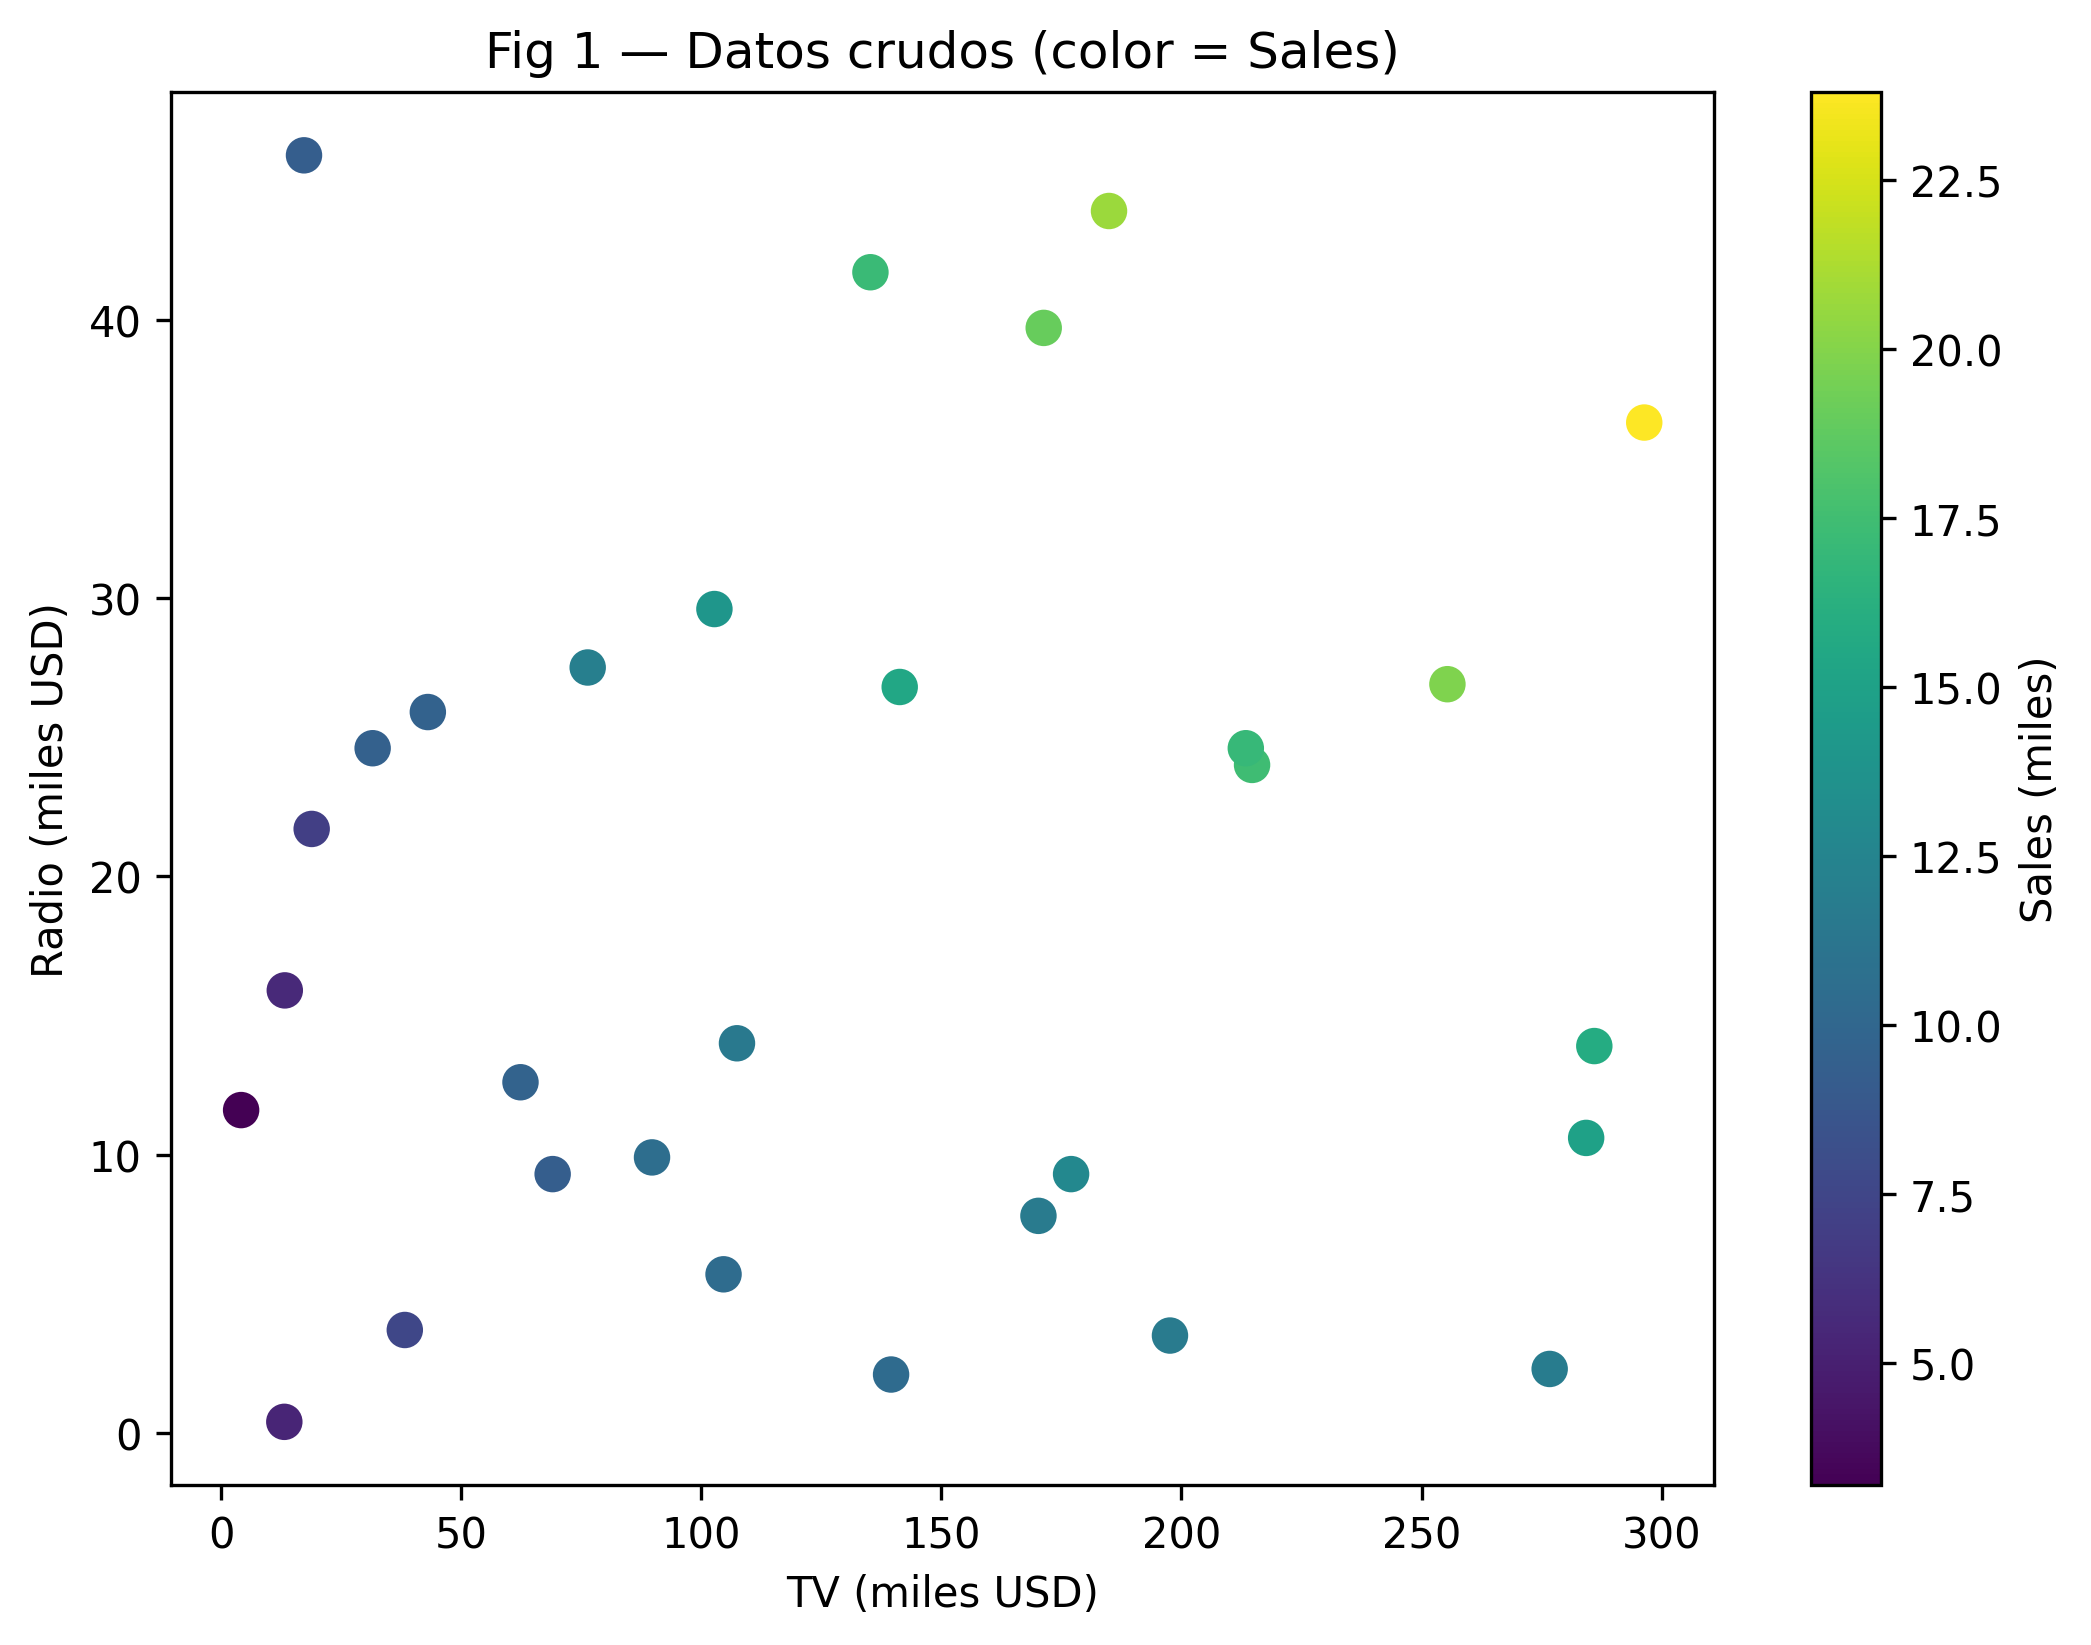
\includegraphics[width=0.75\textwidth]{04_marco_teorico/images/fig1_datos_crudos.png}
\caption{Distribución original de los datos en el plano TV--Radio.}
\label{fig:datos_crudos}
\end{figure}

El primer paso del algoritmo consiste en elegir el corte que maximiza la
reducción de impureza. La Figura~\ref{fig:split1} muestra el primer split
seleccionado en el nodo raíz.

\begin{figure}[H]
\centering
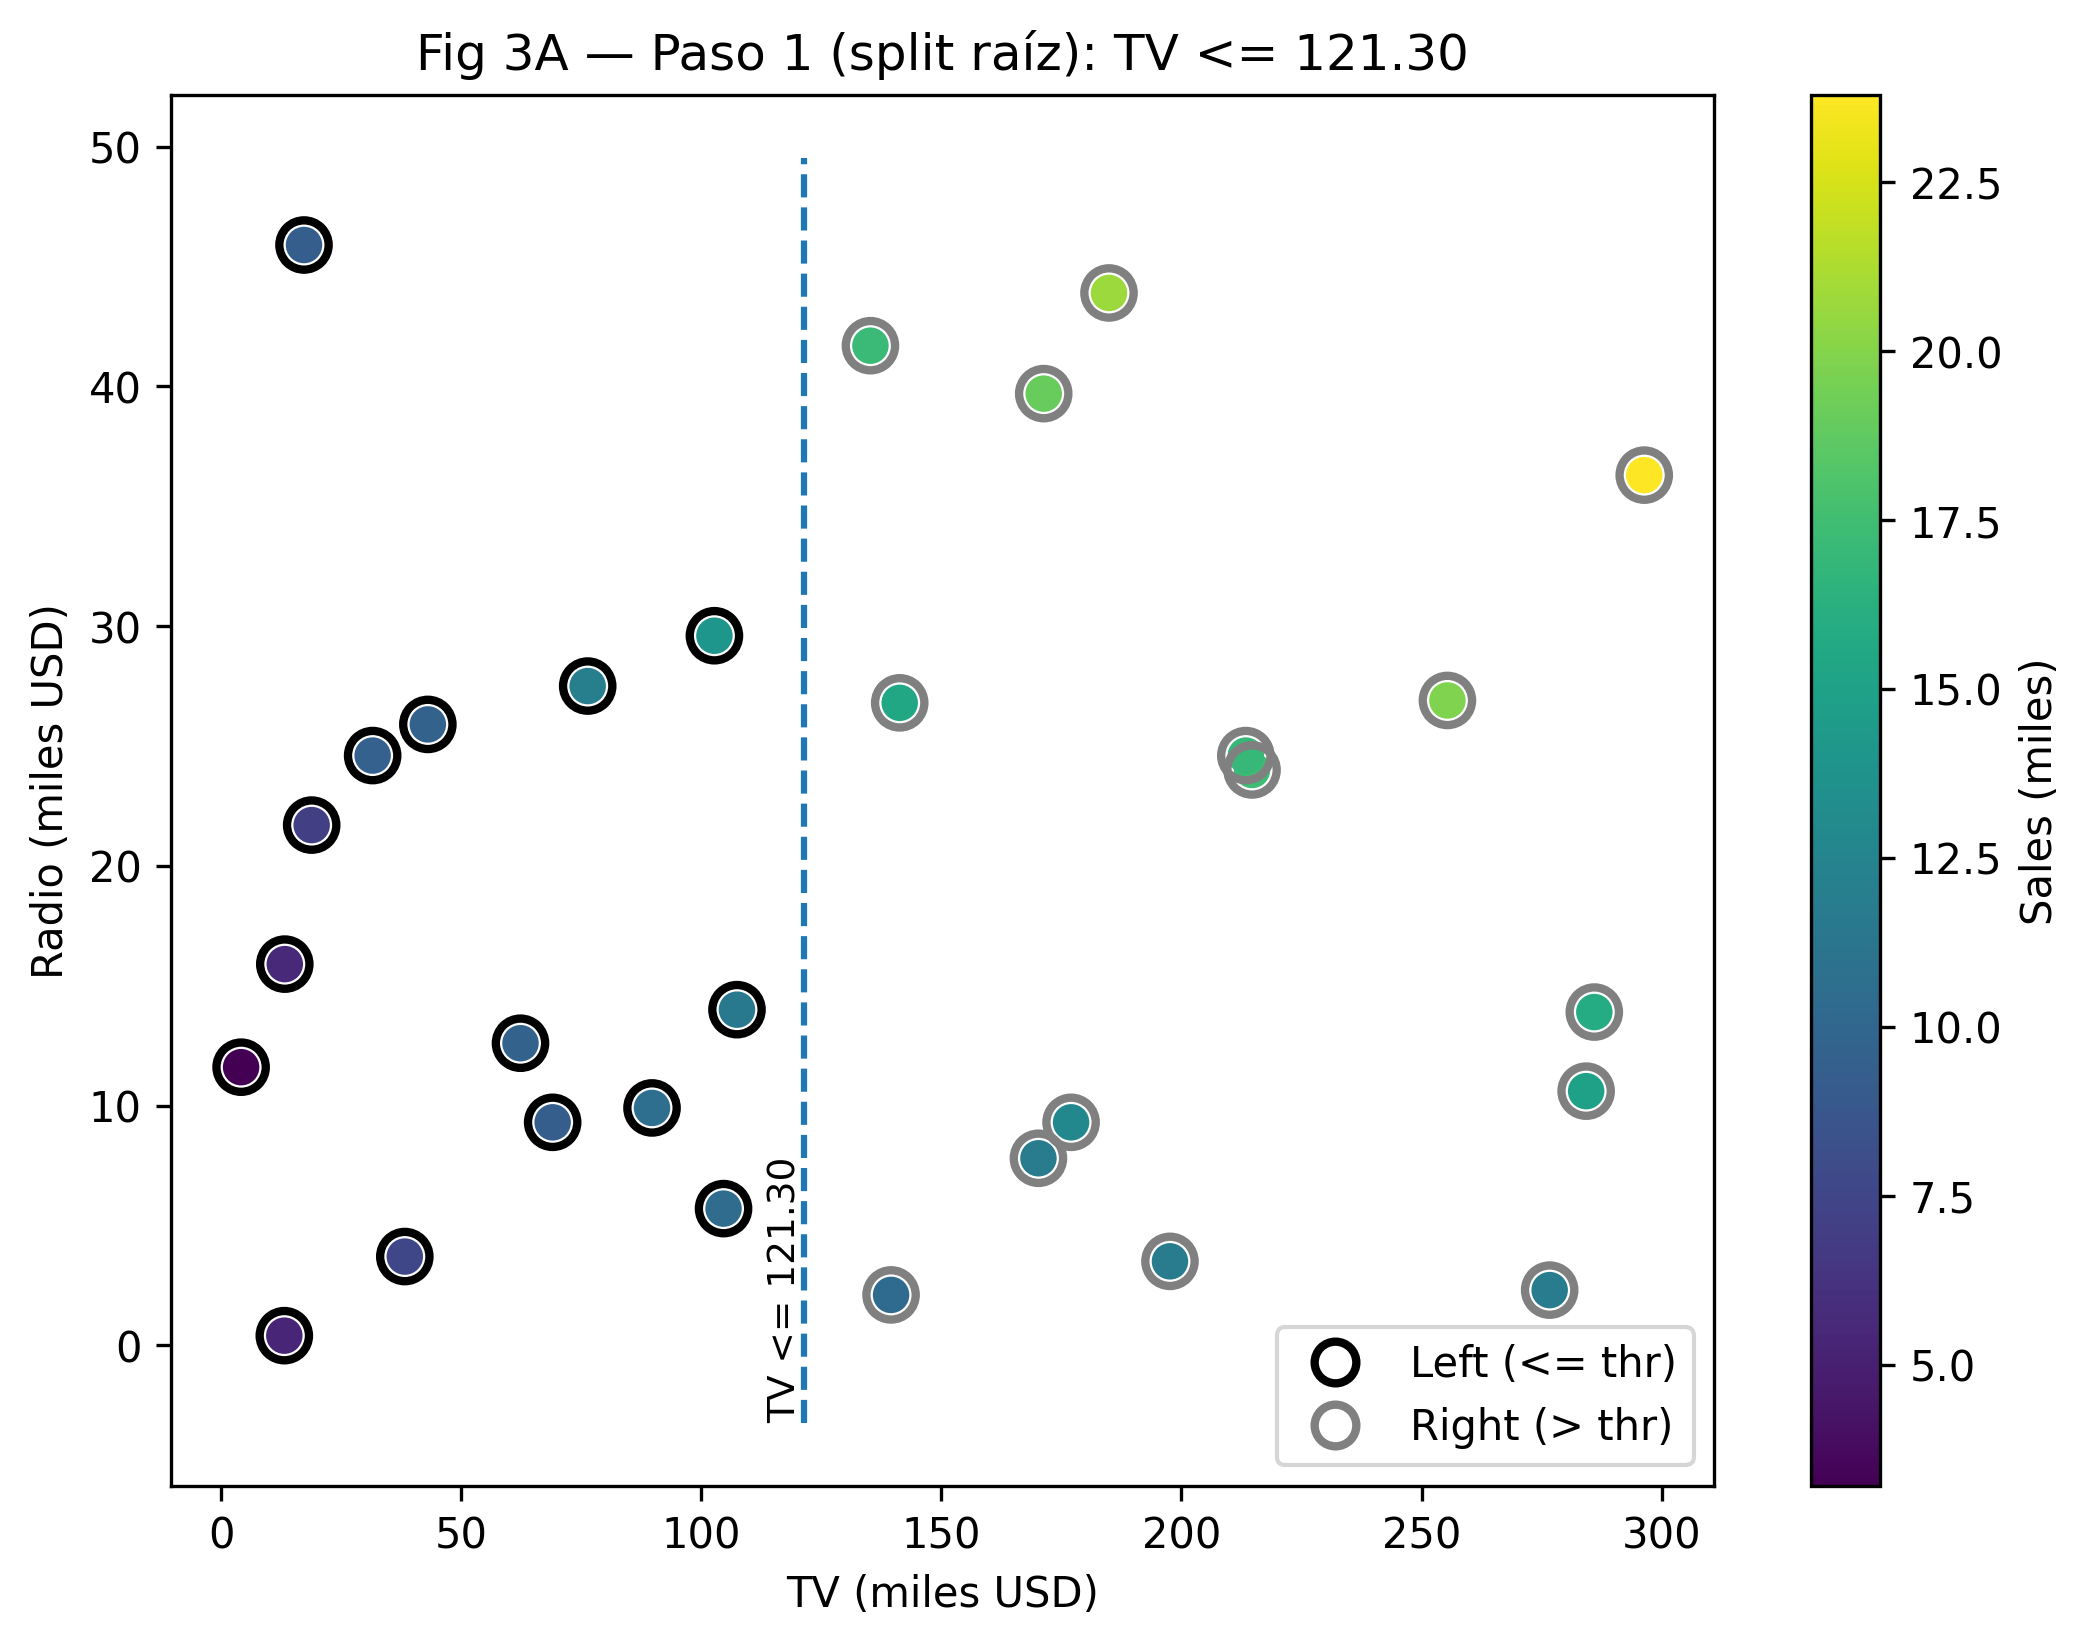
\includegraphics[width=0.75\textwidth]{04_marco_teorico/images/fig3A_paso1_split_raiz.png}
\caption{Primer split seleccionado por el árbol.}
\label{fig:split1}
\end{figure}

En este caso, el algoritmo selecciona una división sobre la variable TV,
con un umbral aproximado de 121.3. Esta recta vertical separa el conjunto de
datos en dos regiones: a la izquierda, observaciones con menor inversión en
televisión, y a la derecha, aquellas con mayor inversión. La elección de este
corte se debe a que produce la mayor reducción de la varianza de la variable
objetivo (Sales) entre todas las divisiones candidatas evaluadas.

La Figura~\ref{fig:tabla_root} muestra la comparación cuantitativa entre este
corte y una alternativa posible.

\begin{figure}[H]
\centering
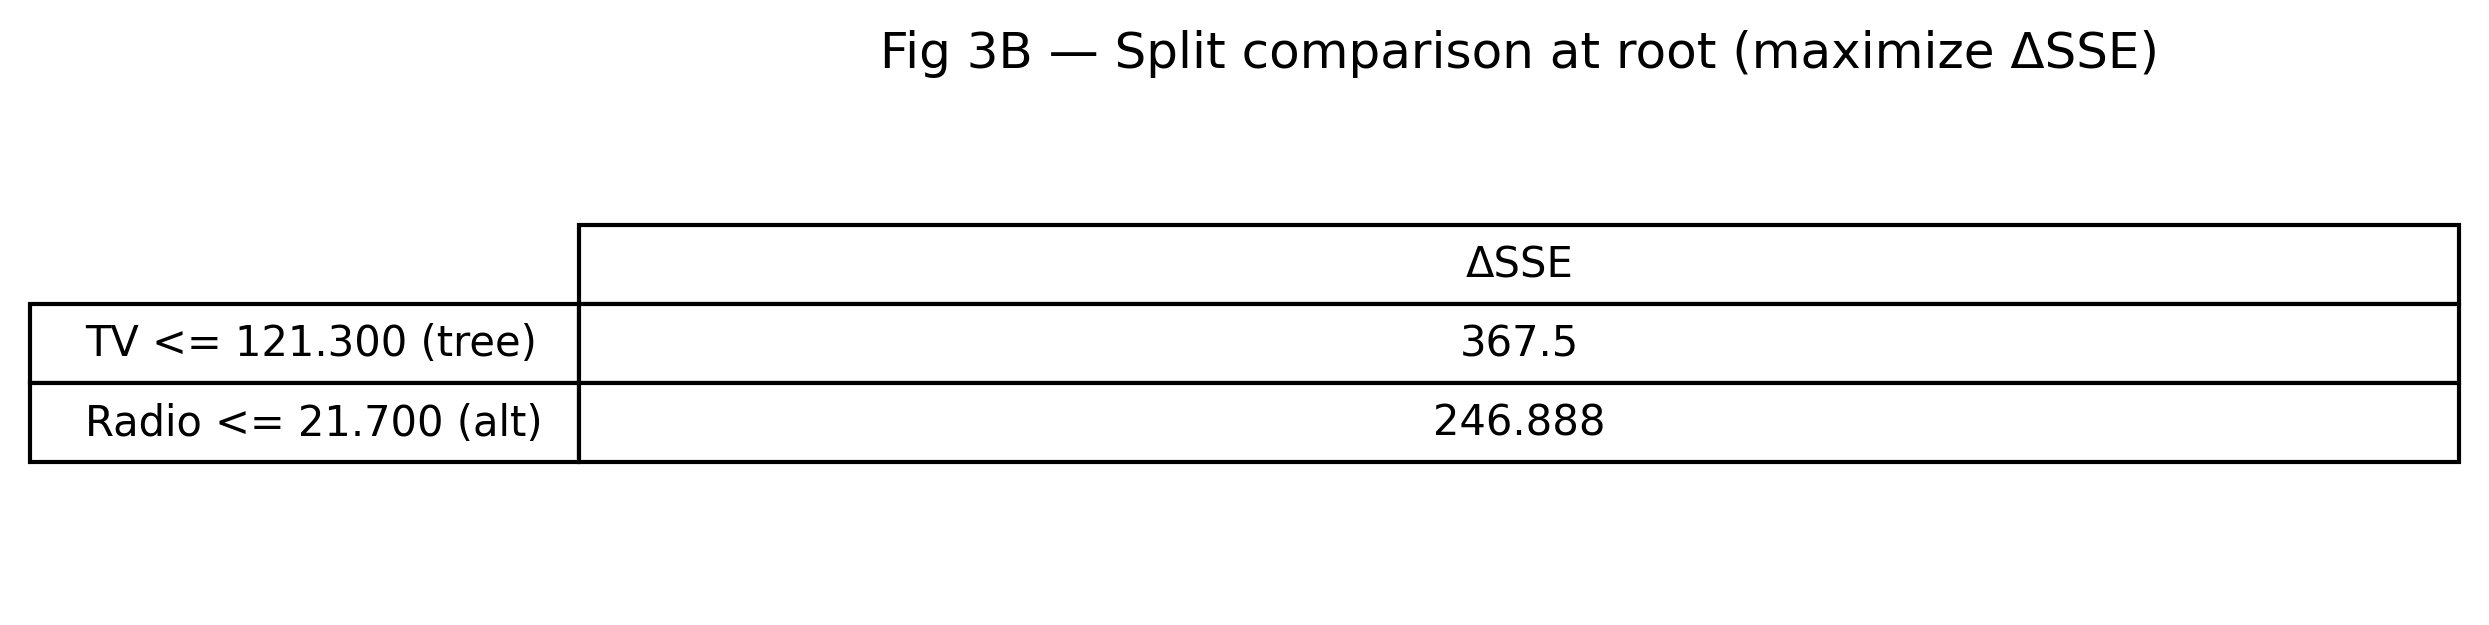
\includegraphics[width=0.9\textwidth]{04_marco_teorico/images/fig3B_tabla_root_vs_alt.png}
\caption{Comparación entre splits en el nodo raíz.}
\label{fig:tabla_root}
\end{figure}

El procedimiento se repite recursivamente. En la Figura~\ref{fig:split23} se
muestran el segundo y tercer corte acumulados, que continúan refinando las
regiones definidas previamente.

\begin{figure}[H]
\centering
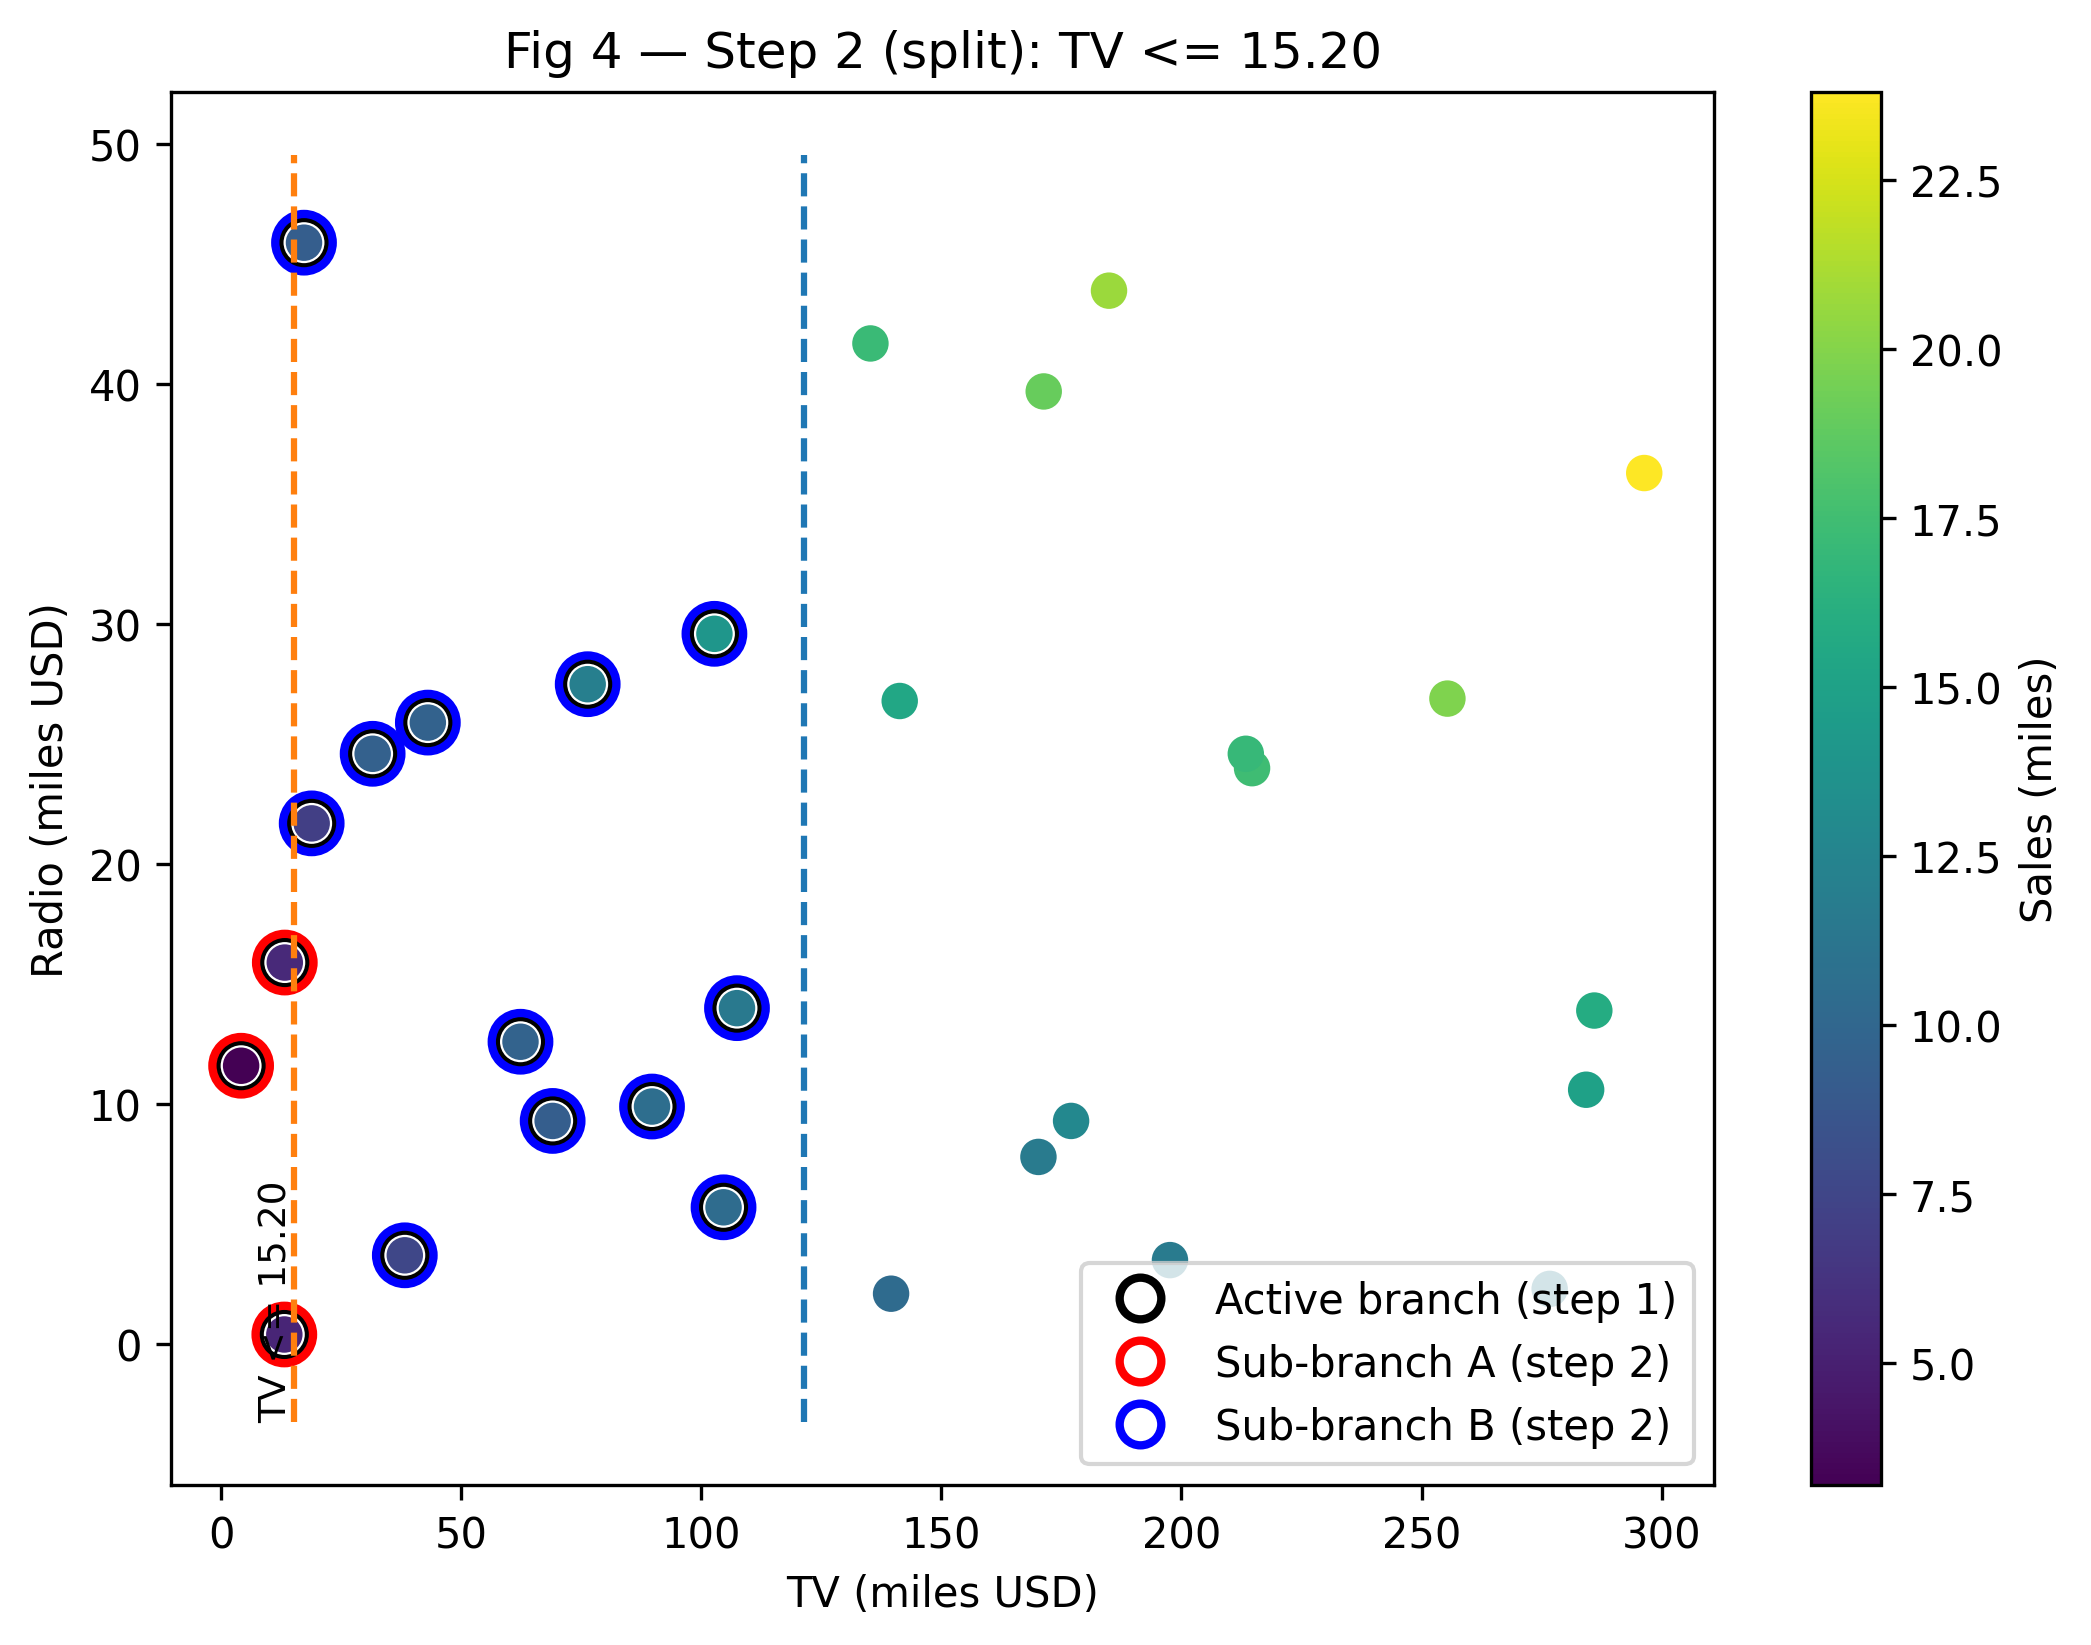
\includegraphics[width=0.5\textwidth]{04_marco_teorico/images/fig4_paso2_split_acumulado.png}\hfill
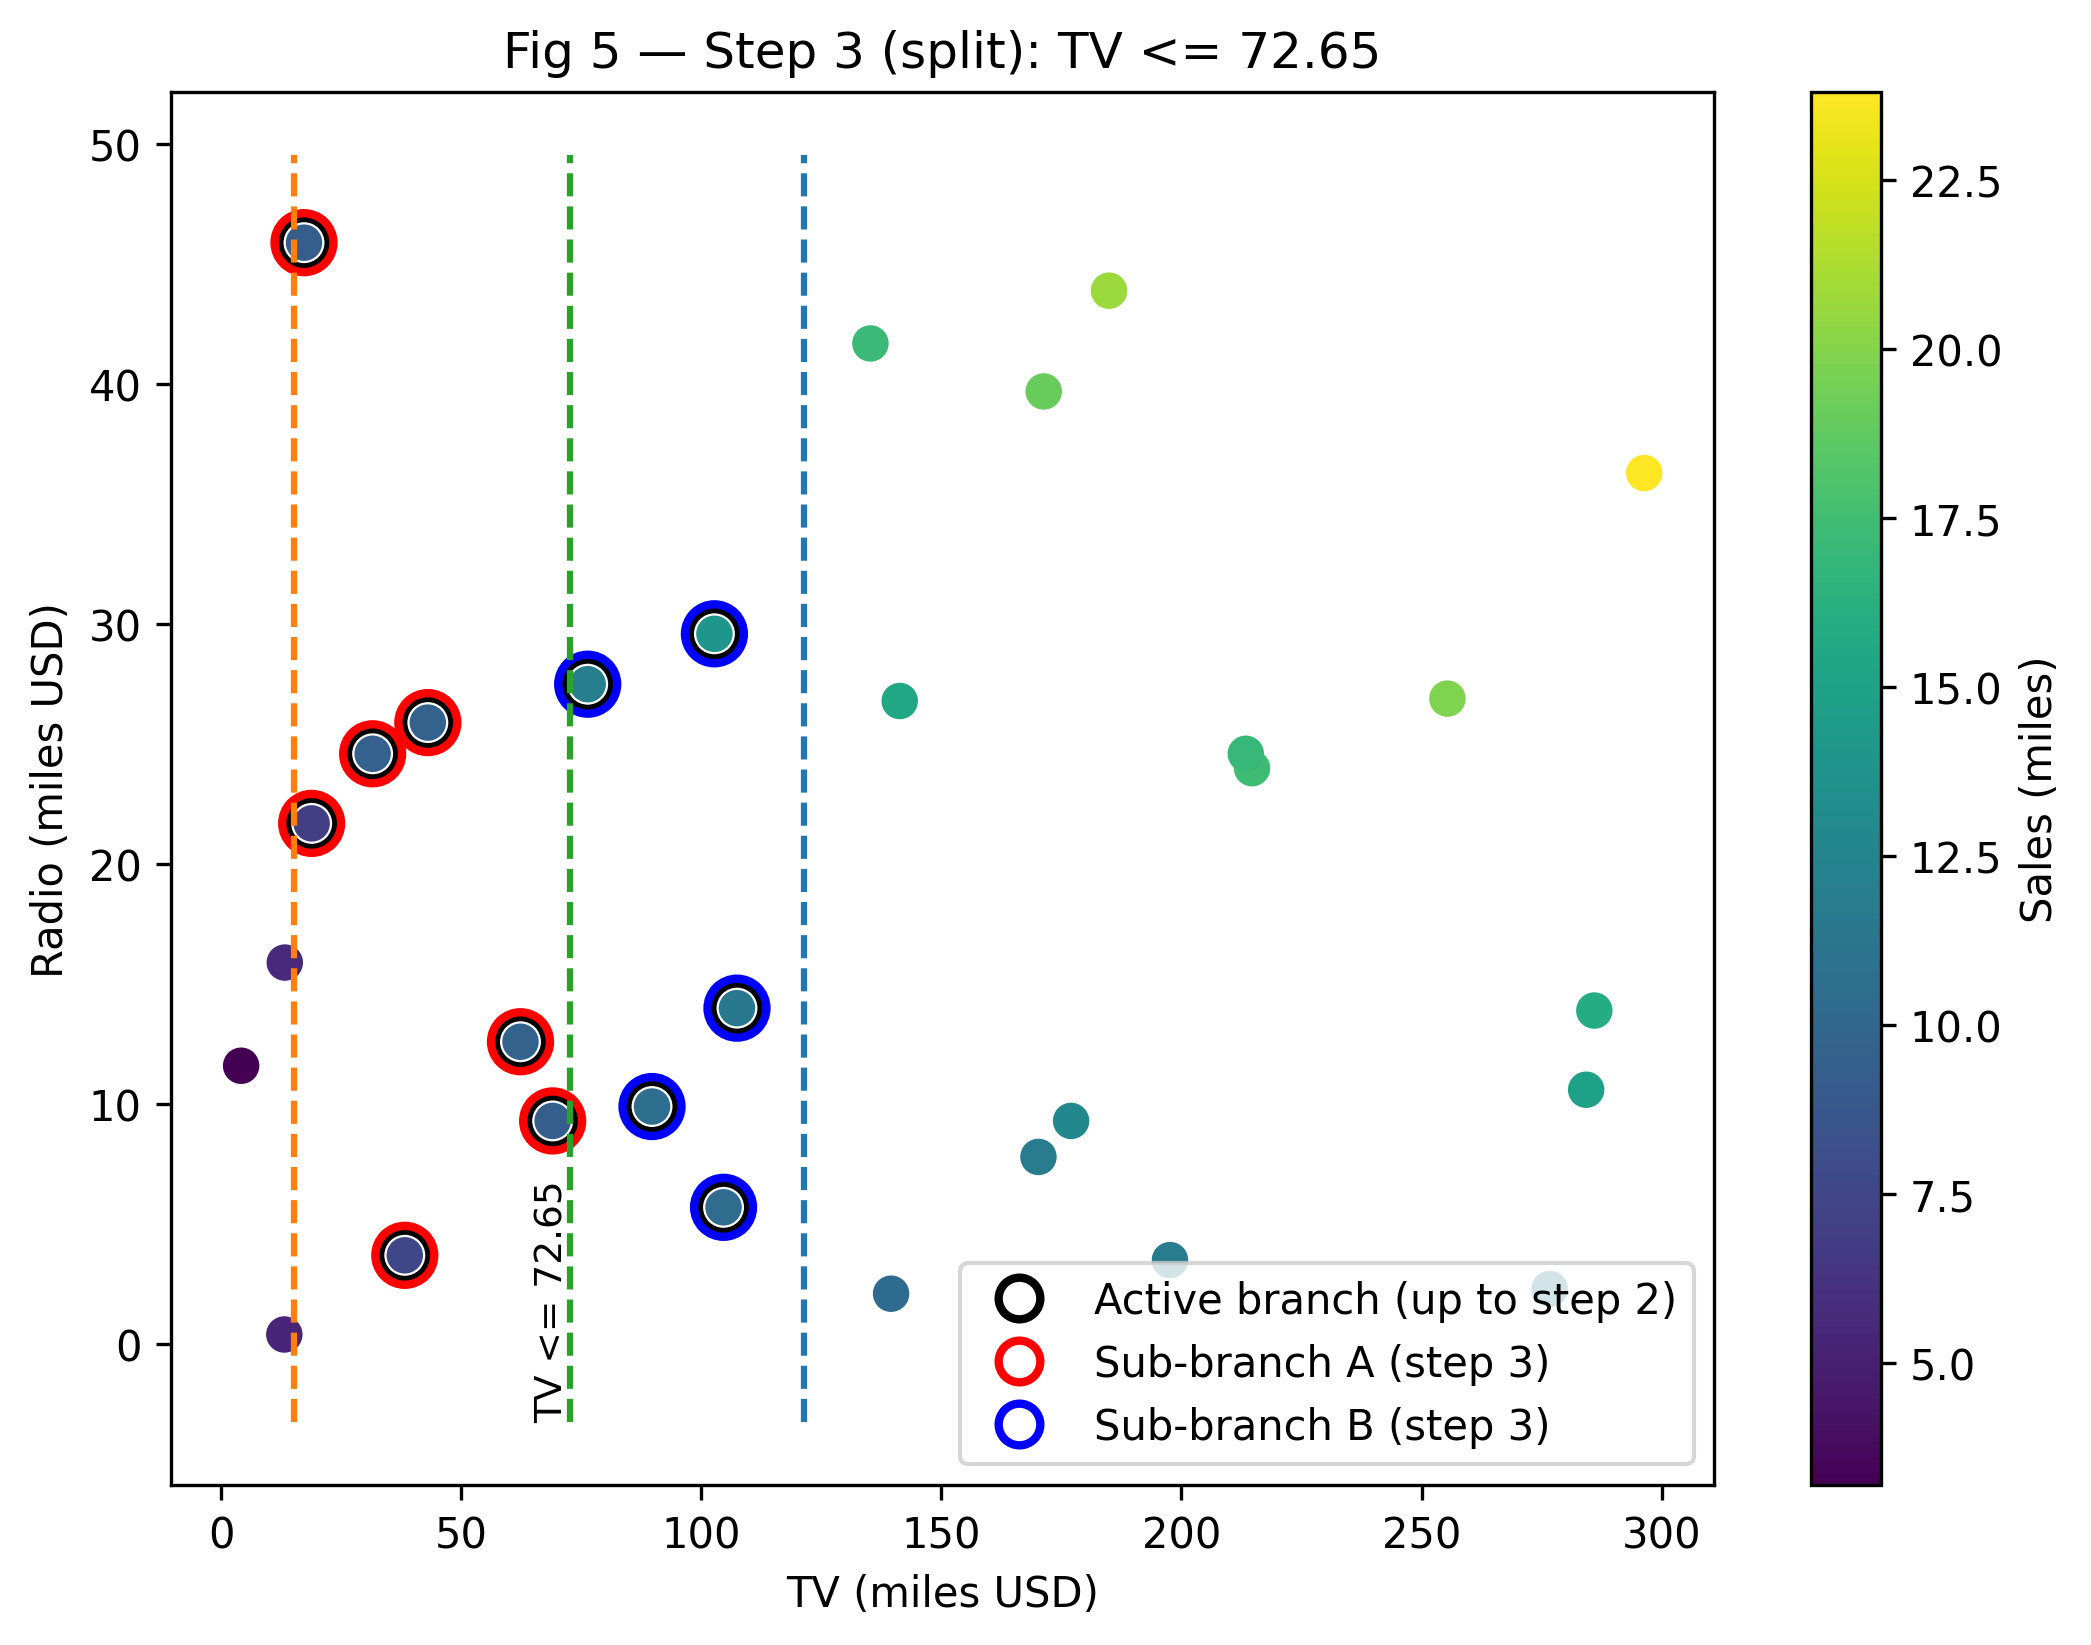
\includegraphics[width=0.5\textwidth]{04_marco_teorico/images/fig5_paso3_split_acumulado.png}
\caption{Segundo y tercer split acumulados.}
\label{fig:split23}
\end{figure}

En este nivel, los nuevos cortes ya no se aplican sobre todo el conjunto de
datos, sino únicamente sobre la región activa heredada del nodo anterior.
De este modo, cada split refina una subregión específica del espacio,
generando particiones cada vez más pequeñas y especializadas.

El resultado final de este proceso es una partición en regiones rectangulares,
donde cada región recibe una predicción constante
(Figura~\ref{fig:regiones}).

\begin{figure}[H]
\centering
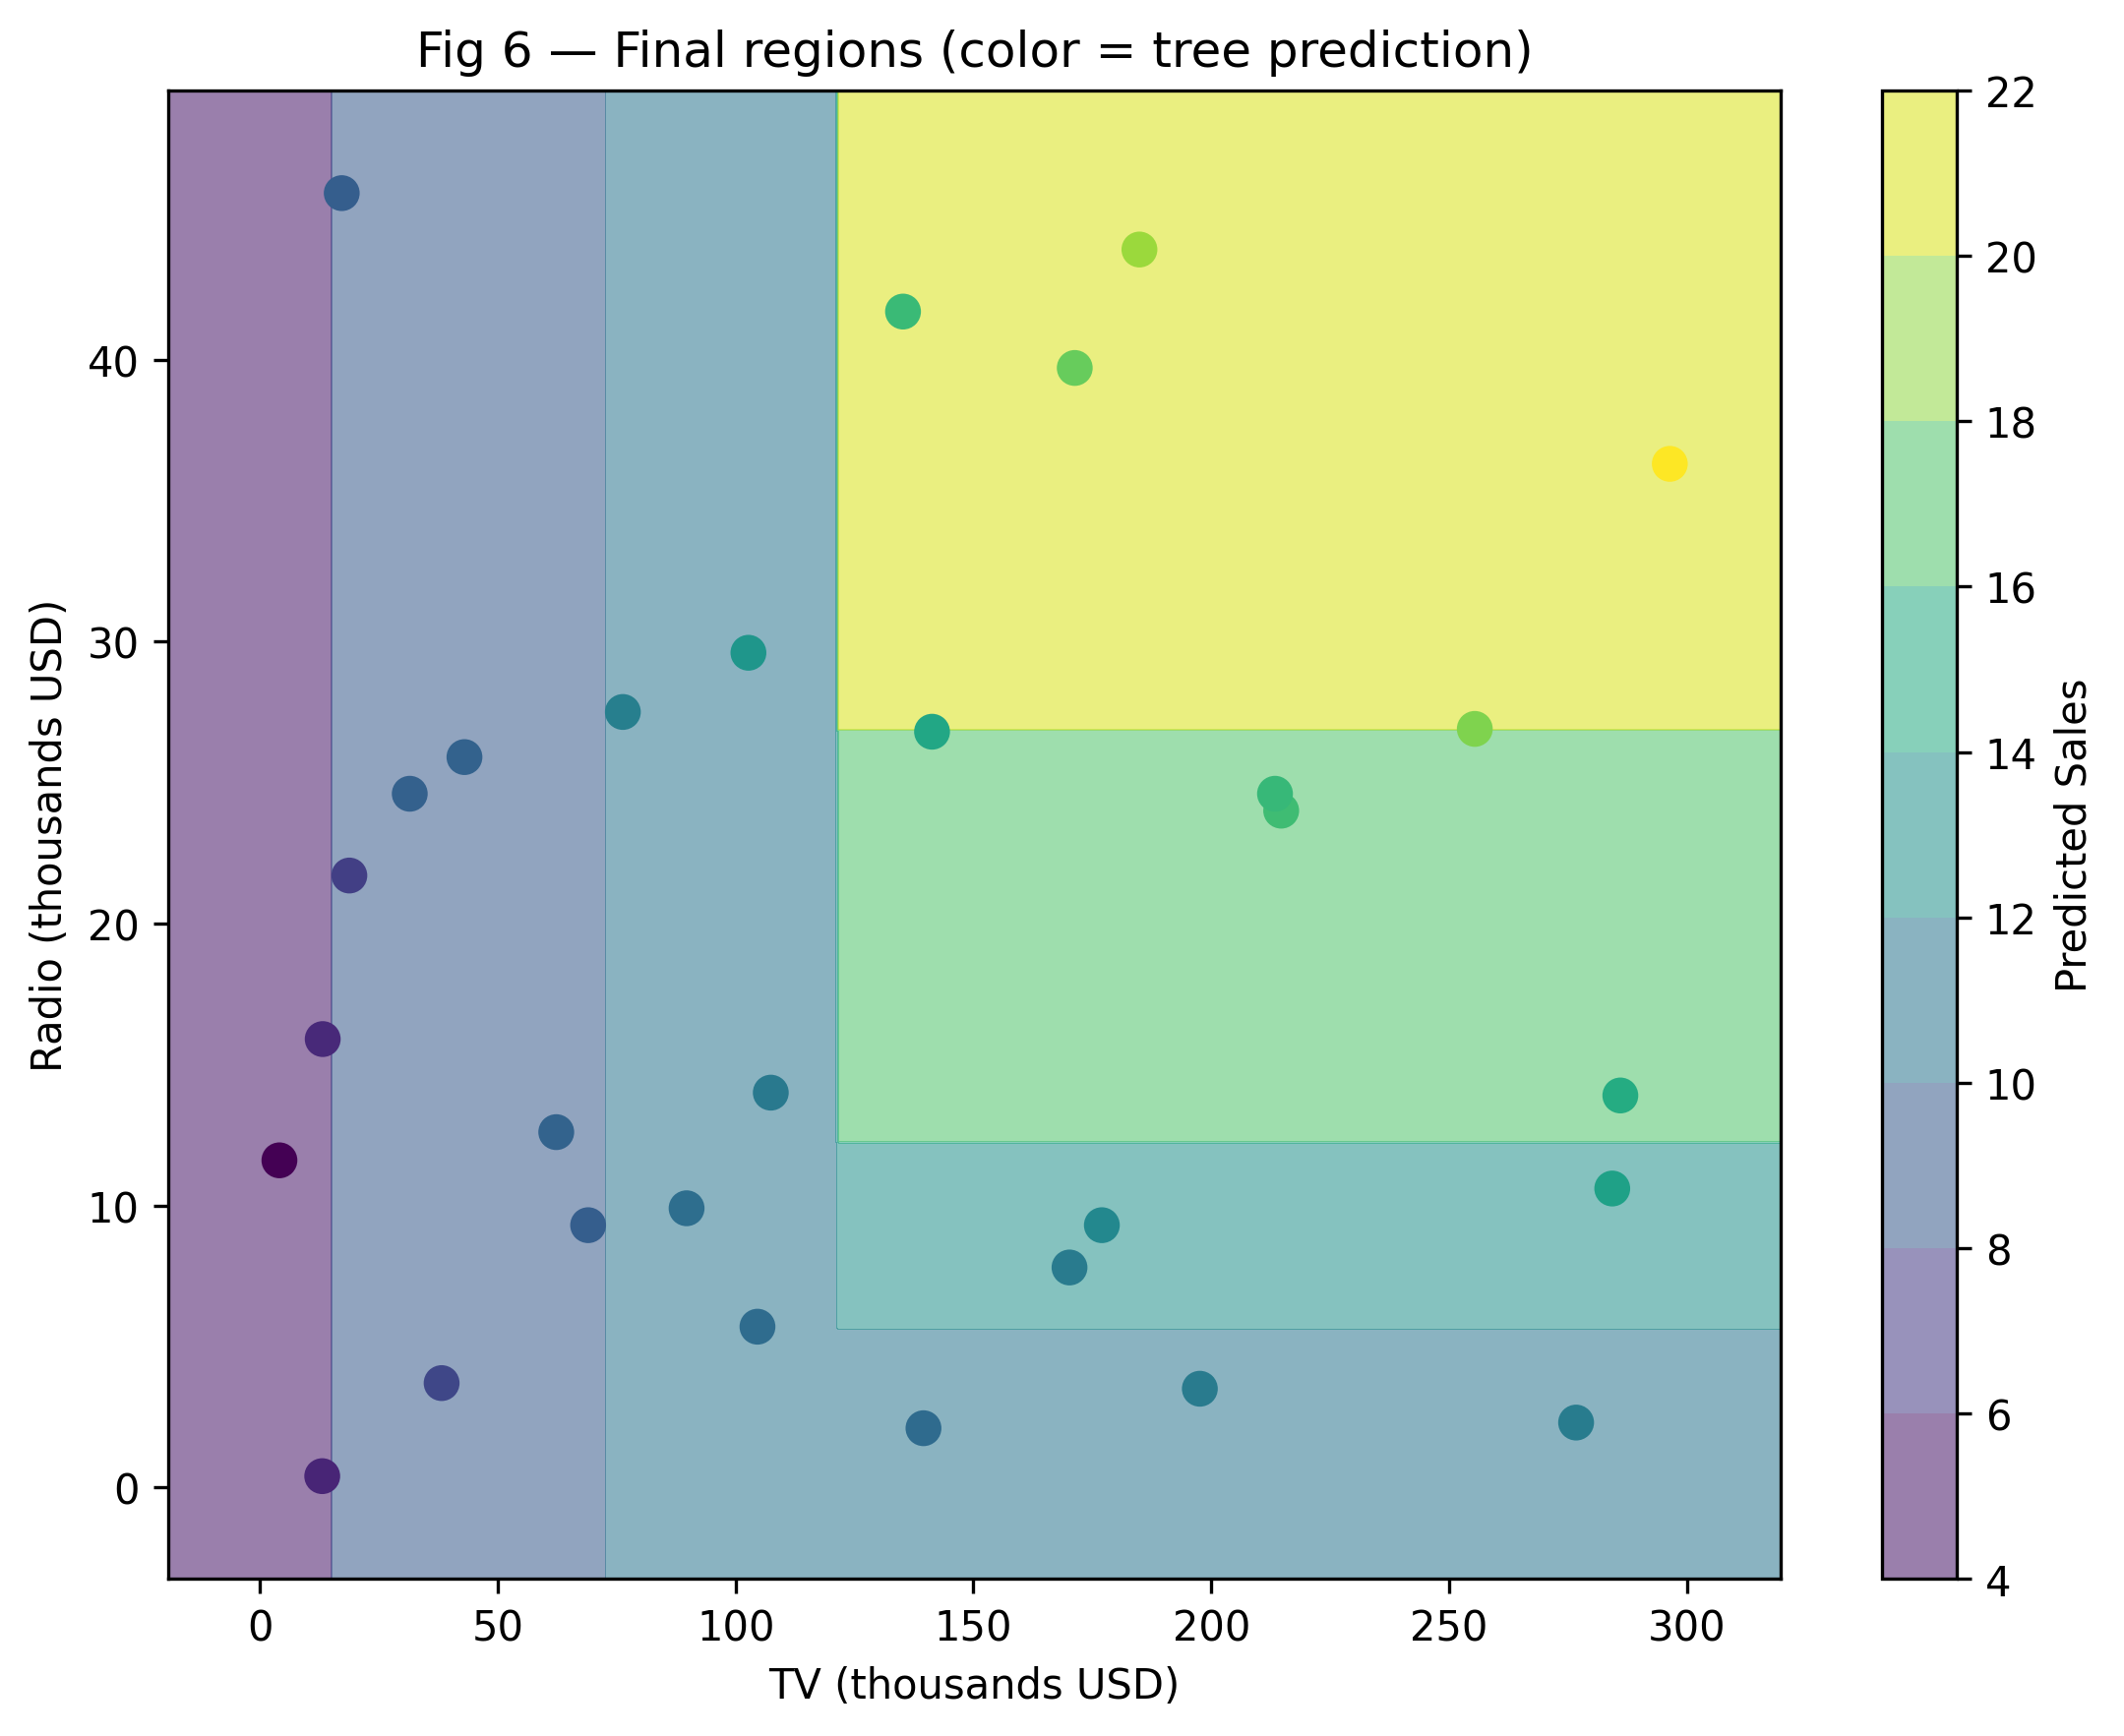
\includegraphics[width=0.75\textwidth]{04_marco_teorico/images/fig6_regiones_finales.png}
\caption{Regiones finales inducidas por el árbol.}
\label{fig:regiones}
\end{figure}

Cada rectángulo coloreado corresponde a una hoja del árbol y representa una
región del espacio de entrada en la que la predicción es constante. El color
indica el valor de predicción (promedio de la variable objetivo) asignado por
el árbol en esa región, de modo que dos puntos ubicados dentro del mismo
rectángulo reciben exactamente la misma salida, independientemente de su
posición específica.

Finalmente, la Figura~\ref{fig:punto} ilustra el recorrido de una observación
nueva hasta una de las hojas, mostrando cómo se obtiene su predicción al
ubicarla en la región correspondiente.

\begin{figure}[H]
\centering
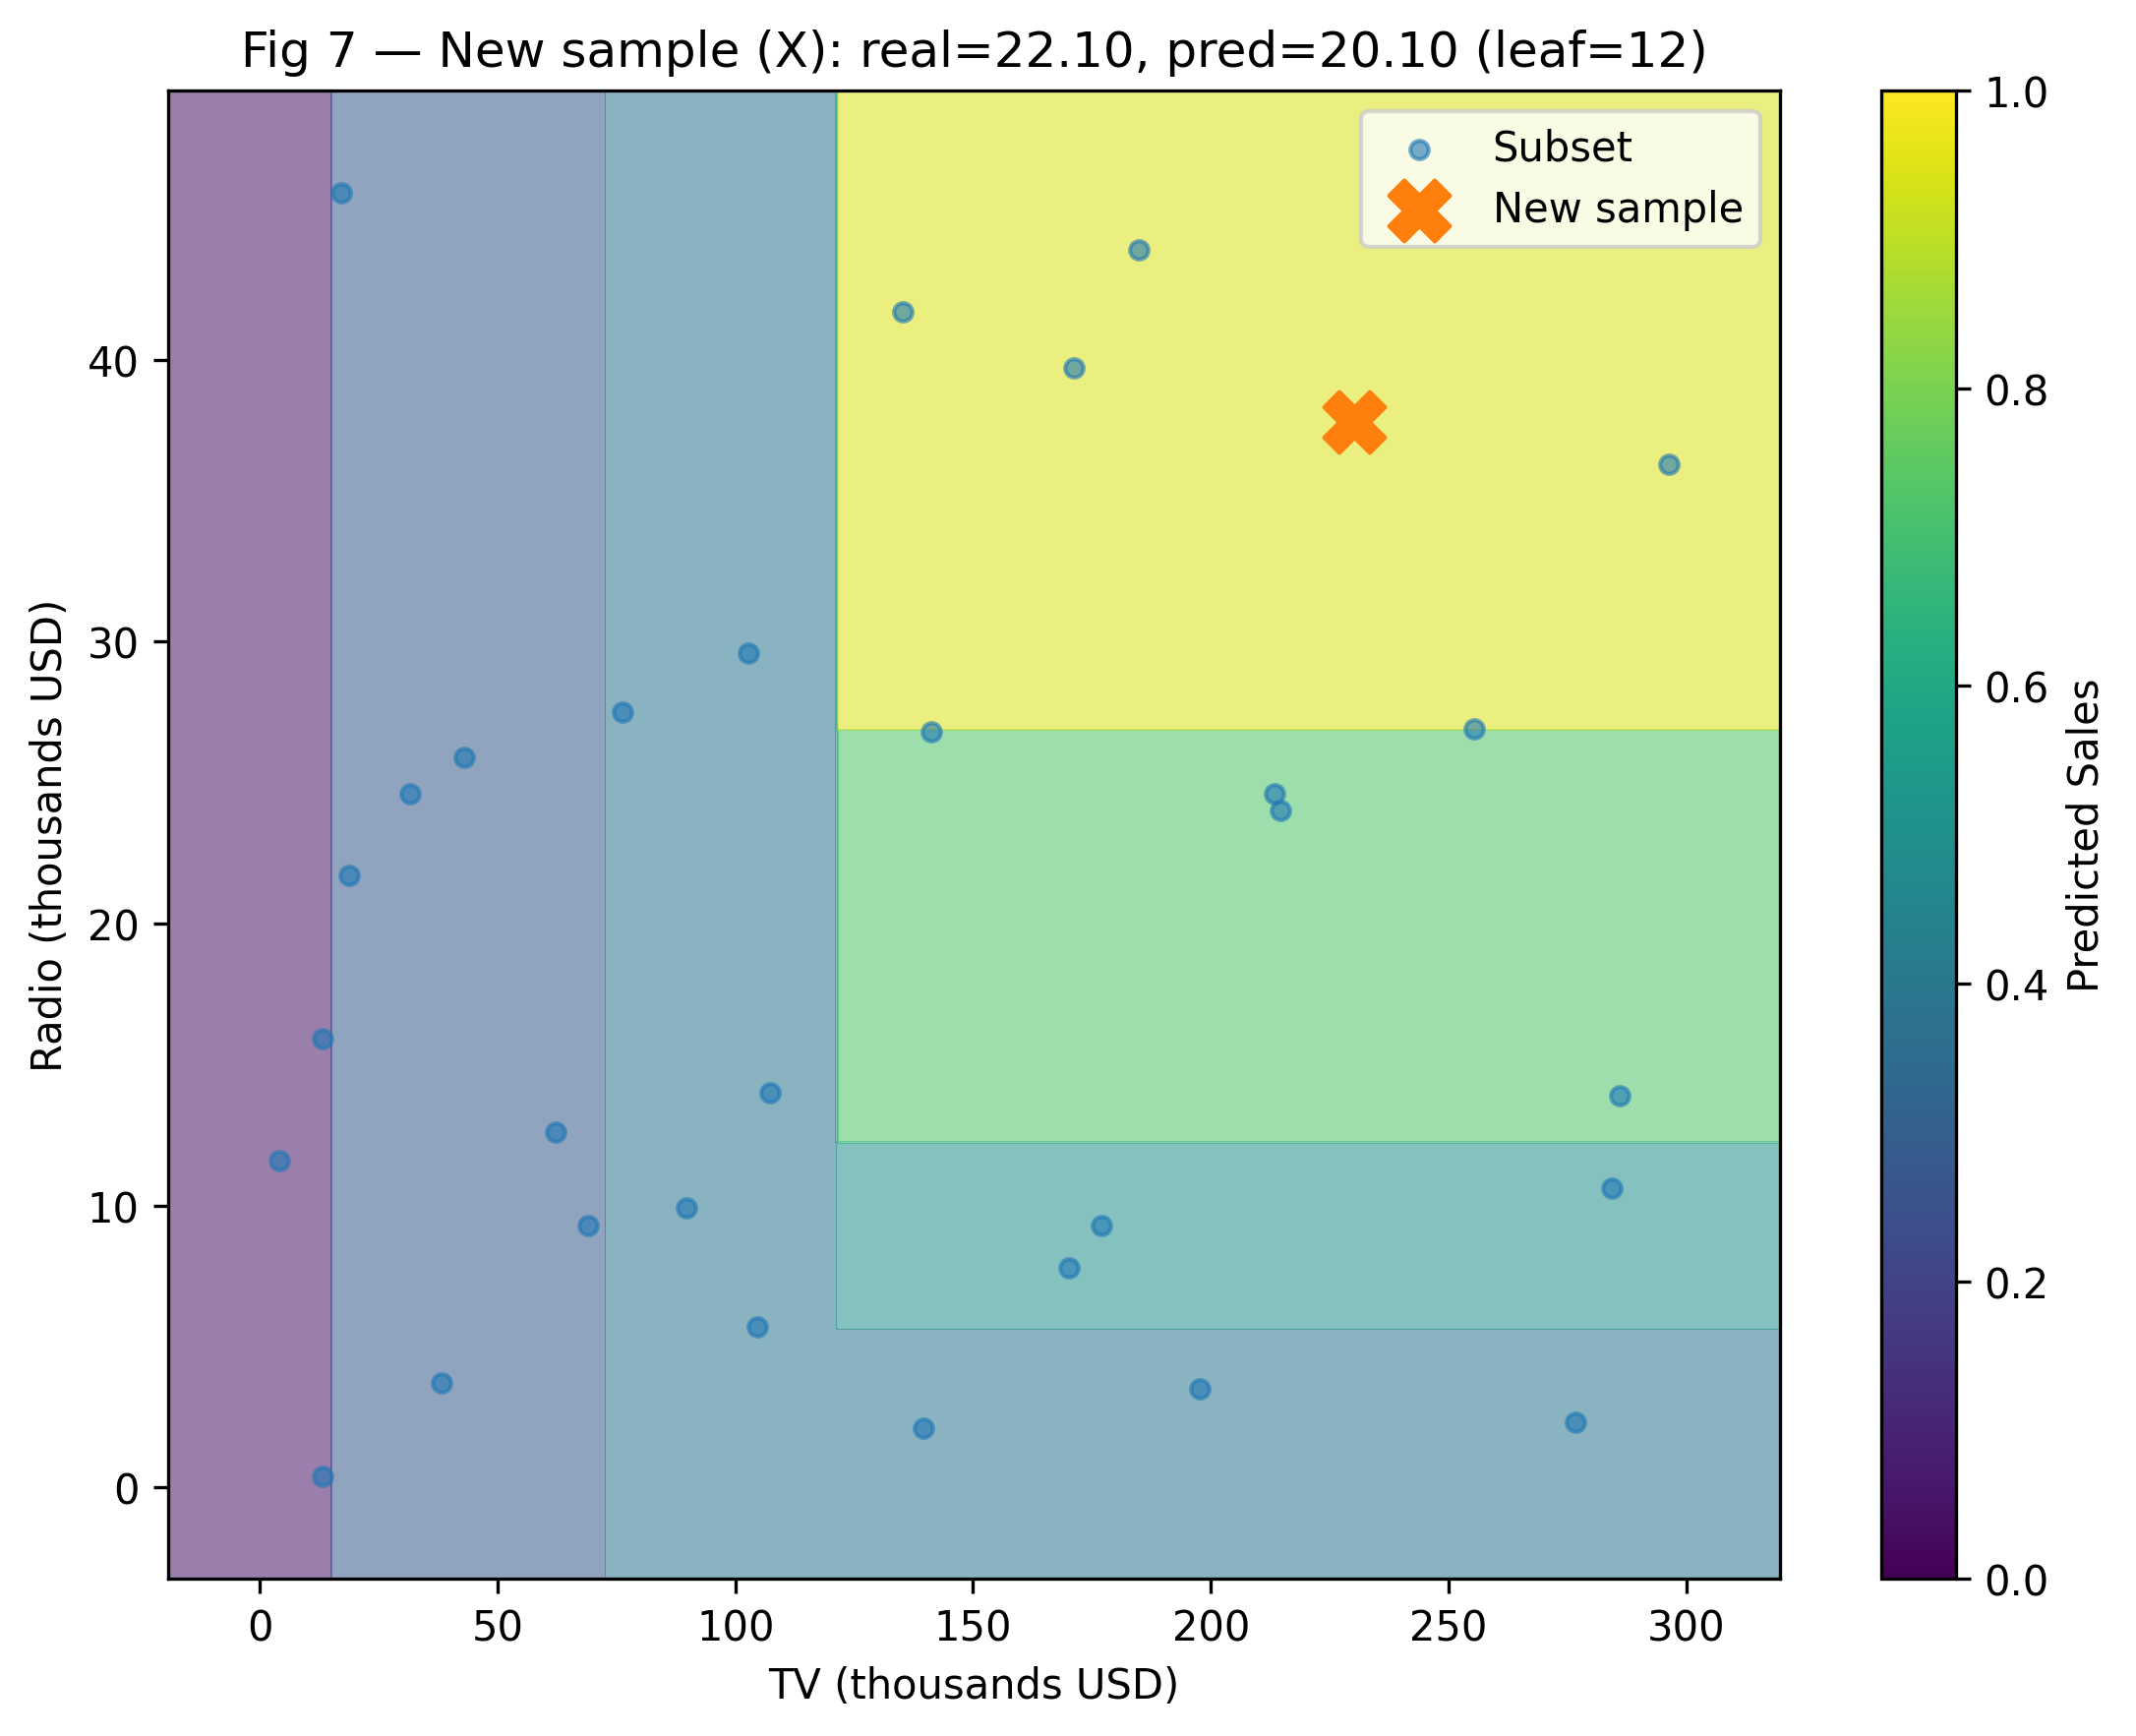
\includegraphics[width=0.75\textwidth]{04_marco_teorico/images/fig7_punto_nuevo_real_vs_pred.png}
\caption{Predicción de un nuevo punto.}
\label{fig:punto}
\end{figure}

Este recorrido resume cómo una partición del espacio de entrada induce una
regla de decisión para cualquier nueva observación. En particular, la región
en la que cae el punto está asociada a una hoja específica del árbol, donde se
almacena el valor de predicción asignado. En el ejemplo mostrado, el modelo
predice $20.1$ frente a un valor real de $22.1$ (error absoluto $=2.0$).

El conjunto completo de reglas generadas por los splits sucesivos queda
codificado en el árbol aprendido, que se muestra en la
Figura~\ref{fig:arbol_completo}.

\begin{figure}[H]
\centering
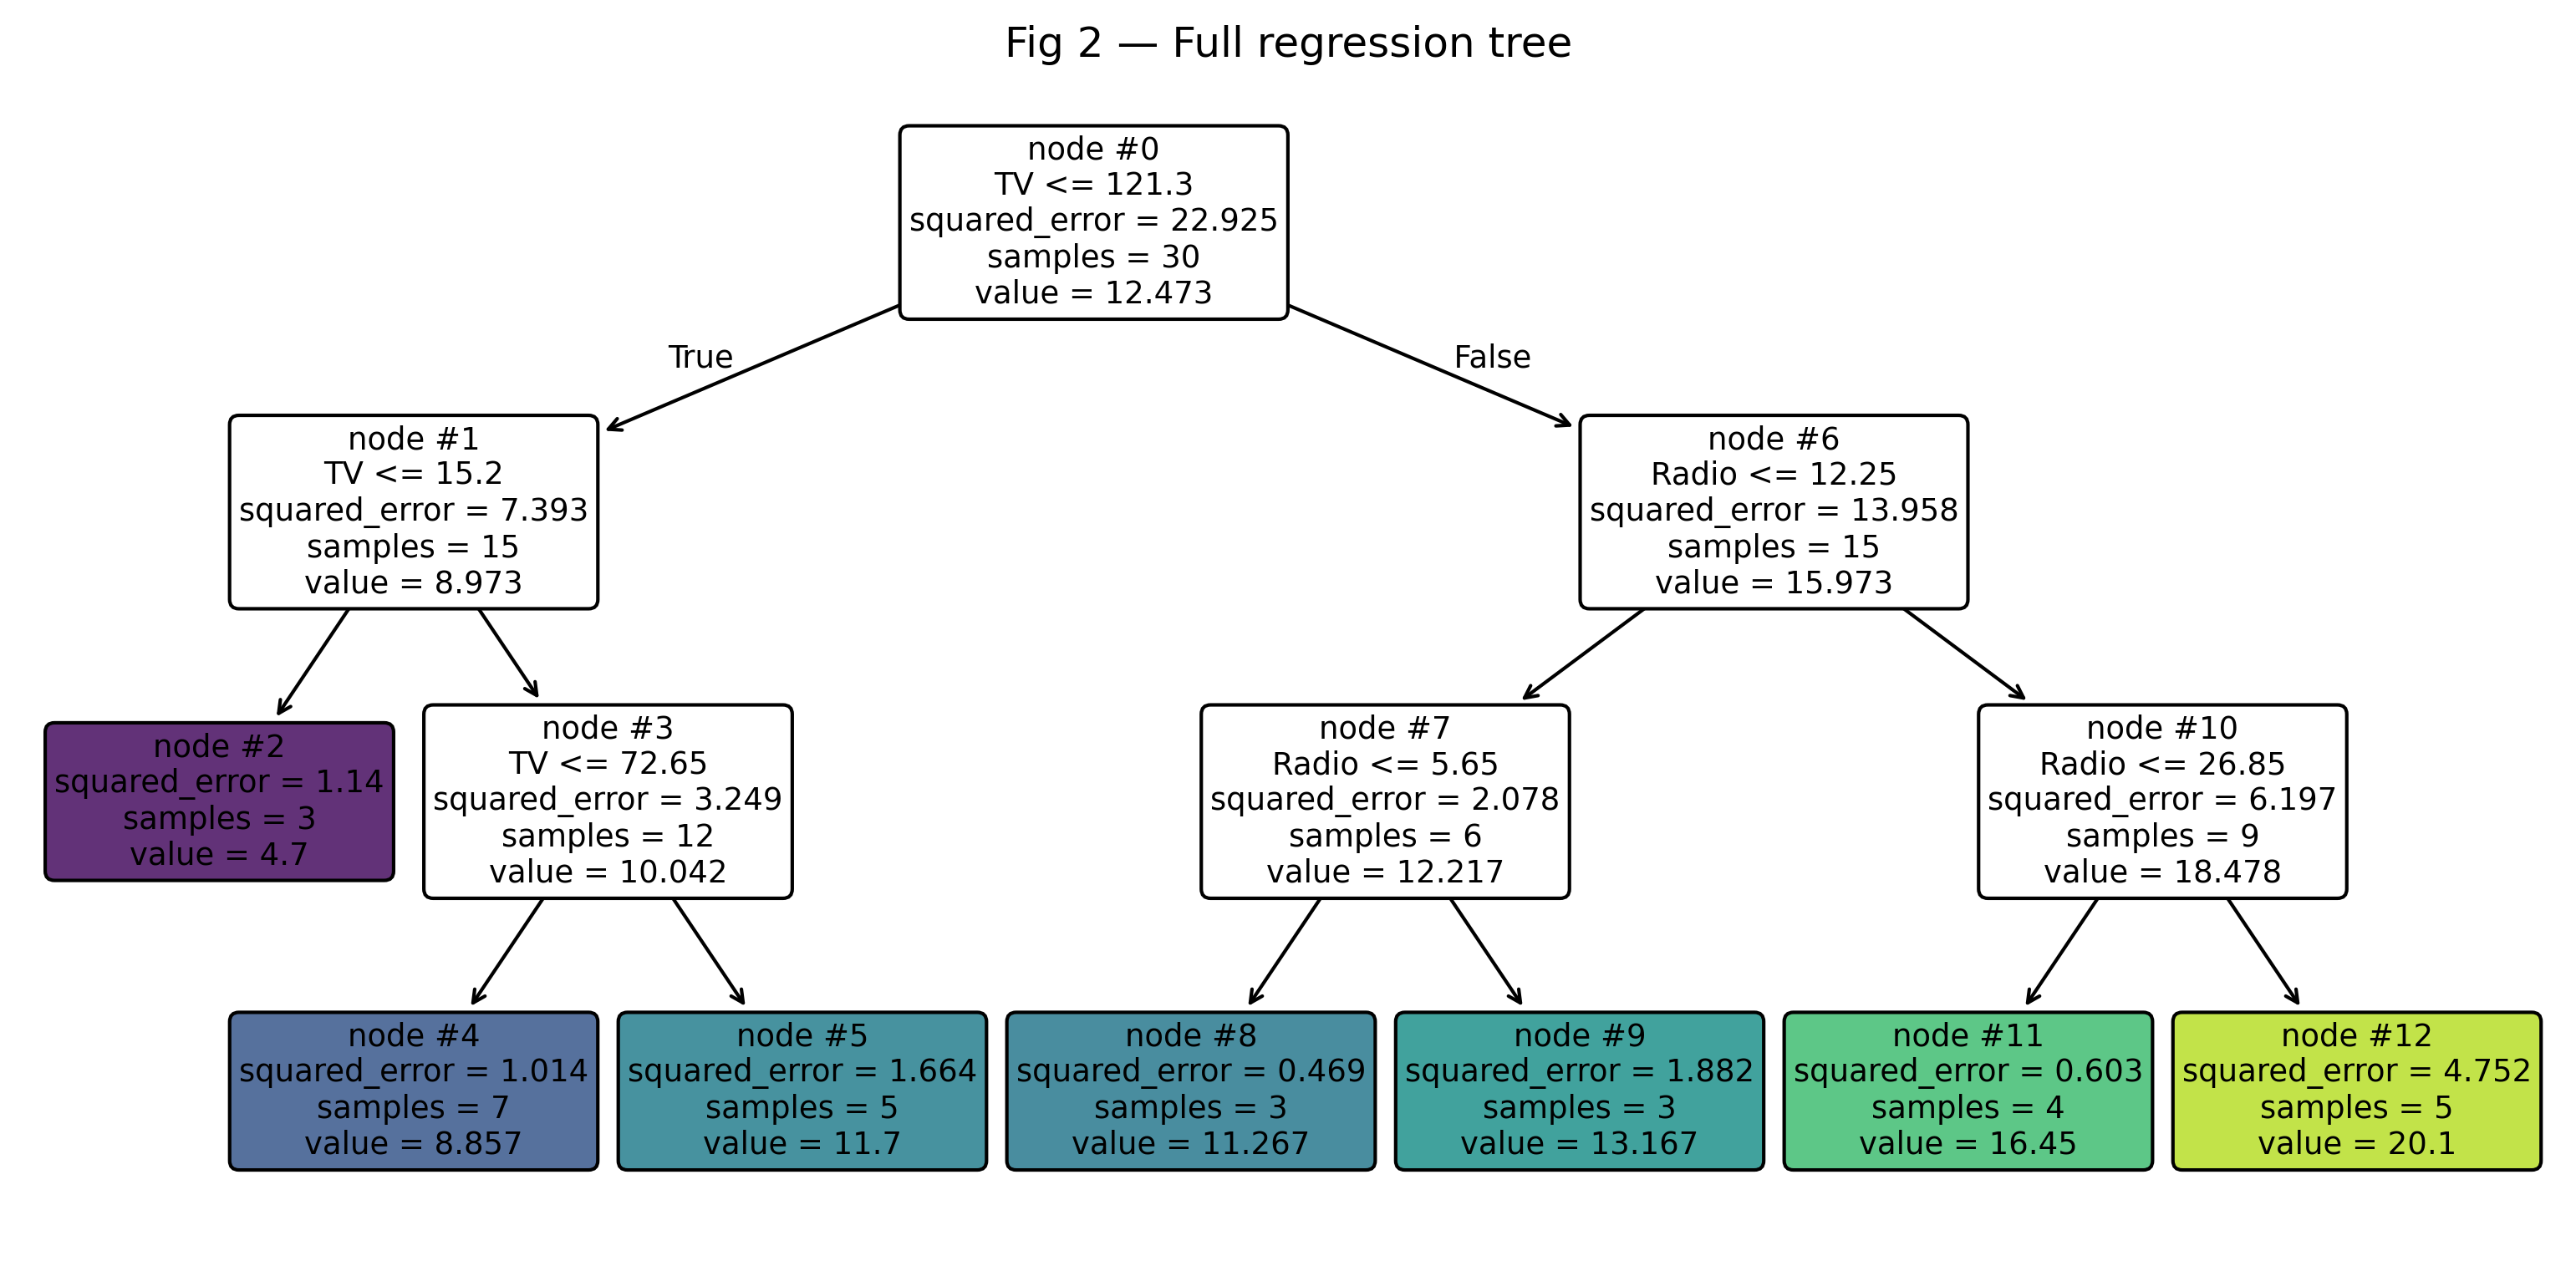
\includegraphics[width=0.99\textwidth]{04_marco_teorico/images/fig2_arbol_completo.png}
\caption{Árbol de regresión completo.}
\label{fig:arbol_completo}
\end{figure}

La estructura del árbol permite visualizar de forma explícita todas las
divisiones aprendidas por el modelo, así como los valores de predicción
asignados en cada hoja.

\medskip

Entre las principales ventajas de los árboles de regresión se encuentra su
capacidad para modelar relaciones no lineales y su interpretación intuitiva.
Sin embargo, presentan una alta tendencia al sobreajuste, ya que pueden
adaptarse excesivamente a los datos de entrenamiento si no se controlan
mediante criterios de parada o regularización. Además, pequeñas variaciones
en los datos pueden producir árboles muy diferentes
\cite{loh2011classification}.

Estas limitaciones motivan el uso de métodos basados en \textit{ensambles},
como el boosting, donde múltiples árboles se combinan para obtener modelos
más robustos, como se describe en la siguiente sección.

\subsubsection{Modelos de ensamble}

Los modelos de \textit{ensamble} combinan múltiples modelos base con el objetivo de obtener un predictor más robusto y preciso que cualquiera de ellos por separado. La idea central es que distintos modelos pueden capturar diferentes aspectos de los datos y que su combinación permite reducir errores y mejorar la capacidad de generalización.

Dentro de este enfoque, existen dos grandes familias: \textit{bagging} y \textit{boosting}, que difieren fundamentalmente en la forma en que se construyen y combinan los modelos.

\paragraph{Bagging.}

Bagging (\textit{Bootstrap Aggregating}) se basa en el muestreo repetido del conjunto de entrenamiento mediante técnicas de \textit{bootstrap}. Dado un conjunto original de $n$ observaciones, se construyen múltiples subconjuntos del mismo tamaño $n$ muestreando con reemplazo. Cada uno de estos subconjuntos contiene los mismos datos originales, pero con repeticiones y omisiones aleatorias.

Sobre cada uno de estos subconjuntos se entrena un modelo independiente, típicamente un árbol de decisión. Este procedimiento se repite muchas veces, generando un conjunto de modelos que, si bien comparten la misma distribución subyacente, presentan diferencias debido al muestreo. La predicción final se obtiene combinando las predicciones individuales, usualmente mediante el promedio en problemas de regresión o el voto mayoritario en clasificación. De este modo, bagging reduce la varianza del modelo y lo hace más estable frente a pequeñas perturbaciones en los datos \cite{breiman1996bagging, hastie2009elements}.
\paragraph{Boosting.}
Boosting sigue una filosofía distinta. En lugar de entrenar modelos independientes, construye una secuencia de modelos de manera iterativa, donde cada nuevo modelo se entrena con el objetivo explícito de corregir los errores cometidos por los anteriores. El procedimiento comienza entrenando un primer modelo sobre el conjunto de datos original. A partir de sus errores, se modifica la distribución de los datos para dar mayor énfasis a las observaciones peor predichas. Con esta versión reponderada del conjunto de entrenamiento se ajusta un nuevo modelo, que intenta corregir las deficiencias del anterior. Este proceso se repite sucesivamente, generando una secuencia de modelos cada vez más especializados en los casos difíciles \cite{schapire1990strength}.

\paragraph{Boosting y teoría PAC.}
Cada uno de los modelos utilizados en boosting es un \textit{weak learner}, es decir, un modelo cuya capacidad predictiva es apenas mejor que la de una predicción aleatoria \cite{kearns1994cryptographic}. En el marco de la teoría PAC (\textit{Probably Approximately Correct}), un algoritmo se considera un weak learner si logra, con alta probabilidad, un error ligeramente menor que el de una elección al azar \cite{valiant1984theory}. A pesar de su debilidad individual, la combinación secuencial de estos modelos permite construir un predictor final considerablemente más potente.

Desde un punto de vista teórico, se demostró que las nociones de
\textit{strong learnability} y \textit{weak learnability} son equivalentes,
es decir, que si una clase de problemas puede ser aprendida por un modelo
fuerte, entonces también puede ser aprendida combinando modelos débiles.
Este resultado fue formalizado por Schapire \cite{schapire1990strength},
resolviendo el denominado \textit{hypothesis boosting problem}.

En este contexto, una \textit{hipótesis} representa el modelo aprendido en
cada iteración, es decir, la función que asigna una predicción a partir de
las variables de entrada.

Una de las primeras construcciones que materializan este resultado fue el
denominado \textit{hypothesis boosting mechanism}, propuesto como una
demostración conceptual de cómo combinar hipótesis débiles para obtener un
clasificador fuerte. En este esquema, se construyen varias hipótesis a partir
de subconjuntos de datos seleccionados de manera adaptativa, es decir,
construidos en función de los errores cometidos por las hipótesis anteriores.
Las predicciones se combinan y se refuerzan aquellas que corrigen los errores
de las anteriores. Si bien este enfoque no fue concebido como un algoritmo
práctico escalable, sentó las bases conceptuales para los métodos modernos de
boosting.

\paragraph{AdaBoost.}
A partir de estas ideas surge \textit{AdaBoost} (Adaptive Boosting), una de las variantes más influyentes de boosting. En AdaBoost, cada muestra del conjunto de entrenamiento posee un peso que se actualiza iterativamente. Al inicio, todas las observaciones tienen la misma importancia. Luego de entrenar un modelo, se incrementan los pesos de las observaciones mal clasificadas y se reducen los de aquellas correctamente clasificadas, de modo que el siguiente modelo se concentre en los ejemplos más difíciles \cite{freund1997decision, freund1999short}. Además, cada modelo entrenado recibe una importancia relativa en la combinación final, de acuerdo con su desempeño.

Si no se utilizan suficientes iteraciones, el modelo resultante puede ser demasiado simple y presentar subajuste. Sin embargo, cuando se emplean modelos base débiles, como árboles de decisión poco profundos, boosting tiende a ser relativamente robusto frente al sobreajuste. 

No obstante, AdaBoost presenta limitaciones importantes en problemas de regresión y en escenarios con ruido o valores atípicos, ya que está estrechamente ligado a una función de pérdida exponencial fija. Esta falta de flexibilidad dificulta su adaptación a tareas donde se requieren otras funciones de error, como la predicción de variables continuas complejas.

\paragraph{Gradient Boosting.}
Otra variante ampliamente utilizada es \textit{Gradient Boosting}, que reformula el
proceso de boosting desde una perspectiva de optimización. En lugar de modificar
explícitamente los pesos de las observaciones, este enfoque utiliza los gradientes
de una función de pérdida para identificar qué ejemplos están siendo peor predichos.

En cada iteración, el nuevo modelo se entrena para aproximar el
\textit{gradiente negativo} de dicha función de pérdida, de modo que el ensamble
completo avanza en la dirección que reduce el error global. Desde este punto de
vista, el proceso puede interpretarse como una optimización por etapas
\cite{friedman2001greedy,natekin2013gradient}.

Una ventaja fundamental de este enfoque es que permite utilizar funciones de
pérdida arbitrarias. Por ejemplo, si se emplea el error cuadrático medio, el
procedimiento equivale a ajustar modelos sucesivos a los errores residuales del
modelo actual \cite{friedman2001greedy,natekin2013gradient}.


Mientras que en AdaBoost las dificultades se reflejan en pesos elevados asignados
a ciertas observaciones, en Gradient Boosting se manifiestan como gradientes de
mayor magnitud.

Sobre esta base, se utilizan variantes modernas de boosting para mejorar
el rendimiento y el control del sobreajuste, entre ellas XGBoost, que será
el modelo supervisado principal en este trabajo y se describe a continuación.

\subsubsection{XGBoost}

La descripción presentada en esta sección se basa principalmente en el trabajo
de Chen y Guestrin \cite{chen2016xgboost}, quienes introducen XGBoost como un sistema de
\textit{gradient tree boosting} orientado a combinar alto rendimiento
predictivo con escalabilidad computacional.

XGBoost (eXtreme Gradient Boosting) es un sistema de aprendizaje supervisado
basado en \textit{Gradient Boosting} con árboles de decisión, diseñado para
ofrecer alto rendimiento predictivo y, al mismo tiempo, escalar de manera
eficiente a grandes volúmenes de datos.  

Desde el punto de vista conceptual, XGBoost sigue el mismo principio que
Gradient Boosting: construir un modelo aditivo que combina múltiples árboles
de decisión entrenados de forma secuencial, donde cada nuevo árbol se ajusta
para corregir los errores cometidos por el ensamble actual. En el contexto de
regresión, esto equivale a aproximar progresivamente la función objetivo
mediante pequeños ajustes que reducen el error global.

La principal diferencia con implementaciones tradicionales de Gradient
Boosting es que XGBoost incorpora, de manera explícita, mecanismos de
regularización y una serie de optimizaciones algorítmicas y computacionales
que permiten entrenar modelos más estables y eficientes, especialmente en
escenarios de alta dimensionalidad.

\paragraph{Función objetivo regularizada.}
XGBoost define una función objetivo que combina dos términos:  
(i) una función de pérdida que mide el error entre las predicciones y los
valores reales, y  
(ii) un término de regularización que penaliza la complejidad de los árboles.
  
Este segundo término controla el número de hojas y la magnitud de los valores
predichos en cada nodo, evitando que el modelo se adapte en exceso a los datos
de entrenamiento. De esta forma, XGBoost logra un mejor equilibrio entre
capacidad de ajuste y generalización.

\paragraph{Árboles ajustados a los residuos.}
El entrenamiento comienza con una predicción inicial constante. A partir de
ella, se calculan los errores (o residuos) entre las predicciones actuales y
los valores reales. En cada iteración, se entrena un árbol de regresión que
aproxima estos residuos, y sus predicciones se suman al modelo previo,
escaladas por un factor de aprendizaje.

Por ejemplo, si el modelo subestima sistemáticamente ciertos valores, el
siguiente árbol aprenderá a corregir esa región del espacio de entrada. Este
proceso se repite hasta que el error global deja de disminuir o se alcanza un
número máximo de iteraciones.

\paragraph{Búsqueda eficiente de divisiones.}
Una dificultad central en los árboles de decisión es encontrar, para cada
variable, el punto de corte que mejor separa los datos. En conjuntos grandes,
evaluar todos los valores posibles resulta computacionalmente costoso.

XGBoost utiliza un enfoque aproximado basado en cuantiles: en lugar de probar
todos los cortes posibles, divide cada variable en un conjunto reducido de
intervalos representativos y solo evalúa esos puntos. Para estimar estos
cuantiles sin recorrer todo el conjunto de datos, emplea un algoritmo llamado
\textit{quantile sketch}, que aproxima la distribución de las variables con un
costo computacional muy bajo.

En problemas de clasificación, esta estimación se realiza de forma ponderada,
dando mayor importancia a los ejemplos cuya predicción es más incierta, lo que
permite concentrar el poder del modelo en las regiones más difíciles.

\paragraph{Manejo de datos faltantes y dispersos.}
XGBoost es \textit{sparsity-aware}, es decir, puede manejar valores faltantes de
forma nativa. Cuando una variable contiene valores ausentes, el algoritmo
aprende automáticamente hacia qué rama del árbol debe enviarlos, en función
de qué opción produce menor error. Esta decisión queda almacenada y se aplica
también a nuevos datos.

Este mecanismo resulta especialmente útil en escenarios reales, donde los
datos suelen ser incompletos o dispersos.

\paragraph{Escalabilidad computacional.}
XGBoost fue diseñado para trabajar con grandes volúmenes de datos. Entre sus
principales optimizaciones se incluyen:

\begin{itemize}
  \item Construcción paralela de las divisiones dentro de cada árbol (la evaluación de splits candidatos se distribuye entre múltiples hilos).
  \item Aprendizaje fuera de memoria (\textit{out-of-core}), que permite
  procesar conjuntos de datos que no caben completamente en la memoria RAM.
  \item Acceso eficiente a memoria mediante estructuras de datos que
  priorizan el uso de caché.
  \item Muestreo de observaciones y variables en cada iteración, lo que reduce
  el costo computacional y ayuda a controlar el sobreajuste.
\end{itemize}

\section{Validación, evaluación y optimización de hiperparámetros}
\label{sec:validacion_evaluacion}

\subsection{Partición de datos y validación cruzada}

En problemas de aprendizaje automático, evaluar el rendimiento de un modelo sobre los mismos datos con los que fue entrenado puede llevar a estimaciones excesivamente optimistas del rendimiento real, un fenómeno conocido como sobreajuste. Para obtener una estimación más realista de la capacidad de generalización, los datos se dividen típicamente en al menos dos conjuntos: uno de entrenamiento y uno de test. El modelo se entrena exclusivamente sobre el primero y se evalúa sobre el segundo, que contiene datos no vistos durante el entrenamiento.

Una extensión de esta idea es la \textit{partición holdout} con tres conjuntos: entrenamiento, validación y test. El conjunto de validación se utiliza para la selección de hiperparámetros y decisiones de diseño del modelo, mientras que el conjunto de test se reserva exclusivamente para la evaluación final. Esta separación garantiza que las métricas reportadas no estén sesgadas por las decisiones tomadas durante el desarrollo del modelo.

La \textit{validación cruzada $K$-Fold} es una técnica que permite obtener estimaciones de rendimiento más robustas. Los datos de entrenamiento se dividen en $K$ subconjuntos (folds) de tamaño aproximadamente igual. En cada una de las $K$ iteraciones, uno de los folds se utiliza como conjunto de validación y los $K-1$ restantes como entrenamiento. El rendimiento final se calcula como el promedio de las $K$ evaluaciones. Esta estrategia tiene la ventaja de que cada observación es utilizada exactamente una vez como dato de validación, proporcionando una estimación menos dependiente de una partición particular de los datos \cite{hastie2009elements}.

\subsection{Métricas de regresión}
\label{sec:metricas_regresion}

Para evaluar el rendimiento de modelos de regresión se utilizan diversas métricas que cuantifican la discrepancia entre los valores predichos $\hat{y}_i$ y los valores reales $y_i$. Las métricas más utilizadas incluyen:

\begin{itemize}
    \item \textbf{Error absoluto medio (MAE):}
    \[
    \text{MAE} = \frac{1}{n} \sum_{i=1}^{n} |y_i - \hat{y}_i|.
    \]
    Representa el error promedio en las unidades originales de la variable objetivo (por ejemplo, años). Es interpretable y robusto frente a valores atípicos.

    \item \textbf{Raíz del error cuadrático medio (RMSE):}
    \[
    \text{RMSE} = \sqrt{\frac{1}{n} \sum_{i=1}^{n} (y_i - \hat{y}_i)^2}.
    \]
    Penaliza proporcionalmente más los errores grandes. Siempre se cumple que $\text{RMSE} \geq \text{MAE}$; una diferencia grande entre ambos indica la presencia de errores puntuales de gran magnitud.

    \item \textbf{Coeficiente de determinación ($R^2$):}
    \[
    R^2 = 1 - \frac{\sum_{i=1}^{n} (y_i - \hat{y}_i)^2}{\sum_{i=1}^{n} (y_i - \bar{y})^2},
    \]
    donde $\bar{y}$ es la media de los valores reales. Indica qué proporción de las diferencias individuales en la variable objetivo es capturada por el modelo. Por ejemplo, un $R^2 = 0{,}41$ significa que el modelo explica el 41\% de la variabilidad observada, mientras que el 59\% restante se debe a factores que el modelo no logra capturar. Un valor de $R^2 = 1$ indica predicción perfecta, mientras que $R^2 = 0$ equivale a predecir siempre la media.

    \item \textbf{Correlación de Pearson ($r$):} mide la fuerza de la asociación lineal entre los valores reales y predichos, complementando al $R^2$ con información sobre la dirección y linealidad de la relación.
\end{itemize}

\subsection{Optimización de hiperparámetros}
\label{sec:hpo_theory}

Los modelos de aprendizaje automático dependen de hiperparámetros que no se aprenden durante el entrenamiento sino que se fijan antes de éste, como la tasa de aprendizaje, la dimensión del espacio latente de un autoencoder o la profundidad máxima de un árbol de decisión. La selección de estos hiperparámetros tiene un impacto significativo en el rendimiento del modelo.

Existen diversas estrategias para la búsqueda de hiperparámetros. La búsqueda en grilla (\textit{grid search}) evalúa todas las combinaciones posibles de un conjunto discreto de valores, pero resulta computacionalmente costosa cuando el número de hiperparámetros es grande. La búsqueda aleatoria (\textit{random search}) muestrea configuraciones al azar del espacio de búsqueda, lo que puede ser más eficiente en espacios de alta dimensión.

Los métodos de optimización bayesiana representan un enfoque más sofisticado que modela la relación entre los hiperparámetros y la métrica objetivo mediante un modelo probabilístico. A partir de este modelo, se proponen nuevas configuraciones en regiones del espacio de búsqueda que tienen mayor probabilidad de mejorar el resultado, equilibrando exploración y explotación. Una implementación de este tipo de enfoque es el algoritmo TPE (\textit{Tree-structured Parzen Estimator}), utilizado por frameworks como Optuna \cite{akiba2019optuna}.

La evaluación de cada configuración de hiperparámetros se realiza típicamente mediante validación cruzada sobre el conjunto de entrenamiento, evitando utilizar el conjunto de test para esta selección.